\documentclass[conference]{IEEEtran}
\IEEEoverridecommandlockouts

\usepackage{cite}
\usepackage{amsmath,amssymb,amsfonts}
\usepackage{algorithmic}
\usepackage{graphicx}
\usepackage{textcomp}
\usepackage{xcolor}
\usepackage{booktabs}
\usepackage{multirow}
\usepackage{url}
\usepackage{subcaption}

\def\BibTeX{{\rm B\kern-.05em{\sc i\kern-.025em b}\kern-.08em
    T\kern-.1667em\lower.7ex\hbox{E}\kern-.125emX}}

\begin{document}

\title{Trade-Offs Between Real-Time Inference Latency and Explanation Faithfulness in Credit Risk Scoring: A Reproducible Empirical Benchmark of TreeSHAP, KernelSHAP, FastSHAP, and LIME}

\author{\IEEEauthorblockN{Anar Gadirli}
\IEEEauthorblockA{\textit{Computer Engineering, ZU / BA Programs} \\
\textit{Azerbaijan State Oil and Industry University (ASOIU)}\\
Baku, Azerbaijan \\
anargadirli55@gmail.com}
}

\maketitle

\begin{abstract}
Automated credit risk assessment systems operating under the European Union Artificial Intelligence Act (Regulation (EU) 2024/1689, Annex III Section 5(b)) and GDPR Articles 13--15 and 22, informed by recent CJEU jurisprudence (\textit{SCHUFA Holding}, C-634/21; \textit{Dun \& Bradstreet Austria}, C-203/22), must deliver faithful local explanations while complying with strict microservice Service Level Agreements (SLAs, e.g., $p95 < 50$\,ms). 
In this study, we present a reproducible empirical benchmark evaluating runtime latency, explanation faithfulness, stability, and amortization economics across four Explainable AI (XAI) paradigms: TreeSHAP, KernelSHAP, FastSHAP (amortized neural explainer), and LIME. 
Evaluations are conducted on a validated 150,000-instance credit scoring benchmark utilizing gradient boosted decision trees (XGBoost, LightGBM) and deep multilayer perceptrons (MLP), recording 6,000 timed observations across 12 model-explainer configurations.

Crucially, our findings establish a fundamental \textit{negative result regarding low-dimensional latency trade-offs}: on standard tabular credit scoring features ($d=10$), all 12 configurations satisfy the 50\,ms SLA with 100\% compliance ($L_{\text{xai}} < 8.5$\,ms at median $p50$, with $p99 \le 10.6$\,ms). In this single-inference regime, switching from TreeSHAP to FastSHAP saves merely $1.4$\,ms. Empirical scaling simulations across $d \in \{10, 25, 50, 100\}$ reveal that SLA-driven trade-offs emerge only when $d > 50$ (where KernelSHAP breaches 50\,ms) or under ultra-high-throughput streaming ($>5,000$ QPS). 
Under controlled reference value functions, FastSHAP distilled from an ExactShapley teacher on MLP achieves $\rho_s = 0.880$ (88.0\% Top-1 agreement), resolving baseline confounding artifacts. On the full test set ($N=22,500$) for XGBoost, TreeSHAP and FastSHAP achieve 77.9\% Top-1 match, rising to 83.3\% within the Adverse Action Cohort ($N=2,250$) and 95.4\% for decisive inputs, with Top-3 and Top-4 Jaccard similarities exceeding 80\%. However, under +3.0\,$\sigma$ covariate shift, FastSHAP rank correlation collapses to $\rho_s = 0.116$, highlighting off-manifold surrogate risks. For low-dimensional neural models ($d \le 12$), Exact Shapley runs in $<28$\,ms, providing zero-drift compliance within real-time SLAs.
\end{abstract}

\begin{IEEEkeywords}
Explainable Artificial Intelligence (XAI), Credit Risk Assessment, Inference Latency, Explanation Faithfulness, TreeSHAP, FastSHAP, KernelSHAP, LIME, High-Risk AI, EU AI Act, CJEU Jurisprudence.
\end{IEEEkeywords}

\section{Introduction}
Machine learning algorithms, particularly gradient boosted decision trees (GBDT) and deep neural networks (DNN), have largely superseded traditional logistic scorecards in commercial credit risk evaluation due to their superior non-linear discrimination performance \cite{lessmann2015benchmarking, hand1997statistical}. However, the opacity of these high-capacity models creates substantial regulatory and operational challenges. 

From a regulatory standpoint, credit scoring is explicitly designated as a \textit{High-Risk AI System} under Annex III, Section 5(b) of the European Union Artificial Intelligence Act (Regulation (EU) 2024/1689) \cite{eu_ai_act_2024}. Consequently, credit underwriting systems are legally obligated to provide transparency, traceability, and meaningful explanations regarding the underlying decision logic. These mandates align with the General Data Protection Regulation (GDPR, Regulation (EU) 2016/679) Articles 13(2)(f), 14(2)(g), 15(1)(h), and Article 22 \cite{gdpr_2016}. 
Recent jurisprudence from the Court of Justice of the European Union (CJEU) has substantially clarified these obligations:
\begin{enumerate}
    \item In \textit{SCHUFA Holding} (Case C-634/21) \cite{cjeu_schufa_2023}, the CJEU held that automated scoring falls within the scope of Article 22(1) GDPR whenever third-party lenders draw decisively on that automated score to establish, implement, or terminate a contractual relationship;
    \item In \textit{Dun \& Bradstreet Austria} (Case C-203/22) \cite{cjeu_dun_bradstreet_2025}, the CJEU clarified that under Article 15(1)(h) GDPR, data controllers cannot satisfy their transparency obligations merely through opaque formulas or generic descriptions; rather, they must provide intelligible explanations of the applied principles and personal data, enabling applicants to understand how alterations in their input profile would alter the credit outcome. In the United States, parallel mandates under the Equal Credit Opportunity Act (ECOA, Regulation B, 12 CFR \S~1002.9) \cite{ecoa_reg_b} require creditors to disclose the principal reasons for adverse credit actions. While the statutory provisions do not specify technical XAI metrics, our legal-analytical deduction is that substituting an approximate explainer that alters the primary identified adverse driver (e.g., Top-1 reason code mismatch) exposes lenders to substantial compliance and audit risks.
\end{enumerate}

Concurrently, financial architectures operate across two distinct operational paradigms:
\begin{enumerate}
    \item \textbf{Asynchronous Compliance and Audit Workflows:} In conventional retail banking and credit underwriting, adverse action notices are generated, archived, and communicated asynchronously (often within a statutory 30-day window under ECOA). In this regime, explanation generation is logged in backend data pipelines where latency is not a critical gating factor.
    \item \textbf{Synchronous Real-Time Inference:} In point-of-sale financing (Buy-Now-Pay-Later, BNPL), merchant checkout gateways, and interactive customer counterfactual simulators (where applicants test ``what-if'' financial adjustments in real time), microservices operate under strict Service Level Agreements (e.g., $p95 < 50$\,ms). If generating an explanation introduces computational overhead on the order of seconds, synchronous serving becomes intractable.
\end{enumerate}

Existing literature predominantly investigates predictive accuracy or qualitative interpretability in isolation \cite{ribeiro2016why, lundberg2017unified, molnar2022interpretable}. Crucially, there remains an acute lack of controlled, empirical benchmarking that simultaneously measures:
\begin{enumerate}
    \item High-resolution component-wise latency ($p50$, $p95$, $p99$ percentiles) separating base model prediction ($L_{\text{pred}}$) from attribution generation ($L_{\text{xai}}$);
    \item Scale-invariant, normalized explanation faithfulness ($\mathcal{F}_{\text{norm}}$) alongside paired bootstrap hypothesis testing and empirical baseline bounds;
    \item Direct ground-truth alignment (Spearman $\rho_s$, $\ell_2$ error, Top-$k$ rank overlap) evaluated on identical reference value functions across tree and neural models;
    \item True retraining stability across independent optimization seeds and bounded input noise; and
    \item The operational break-even economics of amortized neural explainers (FastSHAP) evaluated separately per base model architecture.
\end{enumerate}

In this paper, we address this research gap by conducting an end-to-end empirical benchmark across TreeSHAP, KernelSHAP, FastSHAP, and LIME on gradient boosted trees (XGBoost, LightGBM) and Multilayer Perceptrons (MLP). Notably, our findings demonstrate that for low-dimensional credit risk models ($d=10$), all explainers comfortably satisfy 50\,ms SLAs, indicating that latency-faithfulness trade-offs emerge only under high throughput ($>5,000$ QPS), high feature dimensionality ($d > 50$), or interactive multi-query settings.

\section{Related Work}
\subsection{Feature Attribution and Shapley Values}
Shapley values, originating from cooperative game theory, have become the foundational standard for local feature attribution in machine learning through the unified SHAP framework proposed by Lundberg and Lee \cite{lundberg2017unified}. Shapley values represent the unique attribution method satisfying four essential axiomatic properties: efficiency, symmetry, dummy player, and additivity. 

For an arbitrary prediction model $f$ and instance $x \in \mathbb{R}^d$, the marginal contribution of feature $j$ across feature subsets $S \subseteq N \setminus \{j\}$ is defined as:
\begin{equation}
\phi_j(x) = \sum_{S \subseteq N \setminus \{j\}} \frac{|S|!(|N| - |S| - 1)!}{|N|!} \left[ f_x(S \cup \{j\}) - f_x(S) \right]
\label{eq:shapley}
\end{equation}
Evaluating \eqref{eq:shapley} exactly requires $O(2^d)$ model evaluations, rendering brute-force computation intractable.

To circumvent exponential complexity, Lundberg et al. \cite{lundberg2020local} introduced \textit{TreeSHAP}, which optimizes tree path evaluations in polynomial time ($O(TLD^2)$, where $T$ is the number of trees, $L$ is maximum leaves, and $D$ is maximum tree depth). While TreeSHAP achieves rapid inference on tree ensembles, it cannot be applied to non-tree architectures such as deep neural networks. Conversely, \textit{KernelSHAP} \cite{lundberg2017unified} provides a model-agnostic formulation by solving a weighted linear regression over coalition samples, but incurs significant sampling latency ($O(M \cdot n_{\text{samples}})$).

\subsection{Amortized Explanation: FastSHAP}
To resolve the inference-time latency bottleneck of sampling-based explainers, Jethani et al. \cite{jethani2022fastshap} introduced \textit{FastSHAP}. Rather than solving an independent optimization problem for every query instance $x$, FastSHAP amortizes computation by training an auxiliary parameterized neural network $\phi_\theta(x)$ that learns to predict Shapley values in a single forward pass. In model-agnostic settings, FastSHAP minimizes the weighted Shapley kernel loss over subset coalitions $S \subseteq \{1, \dots, d\}$ with Shapley weights $w(S) = \frac{d - 1}{\binom{d}{|S|} |S| (d - |S|)}$:
\begin{equation}
\begin{split}
\mathcal{L}_{\text{FastSHAP}}(\theta) = \mathbb{E}_{x, S} \Biggl[ w(S) \Biggl( \sum_{j \in S} \phi_\theta(x)_j \\
- \Bigl( f(x_S \cup b_{\bar{S}}) - \mathbb{E}[f(X)] \Bigr) \Biggr)^2 \Biggr]
\end{split}
\label{eq:fastshap}
\end{equation}
When ground-truth references $\phi^*(x)$ are accessible during training, FastSHAP is formulated as a student distillation network supervised by both $\ell_2$ MSE and directional cosine ranking loss:
\begin{equation}
\begin{split}
\mathcal{L}_{\text{distill}}(\theta) = \mathbb{E}_{x} \Bigl[ \|\phi_\theta(x) - \phi^*(x)\|_2^2 \\
+ \lambda_{\text{cos}} \bigl(1 - \cos(\phi_\theta(x), \phi^*(x))\bigr) \Bigr]
\end{split}
\label{eq:fastshap_distill}
\end{equation}
where $\cos(u, v) = \frac{u \cdot v}{\|u\|_2 \|v\|_2}$ enforces strict preservation of relative feature risk ranking. In our controlled benchmark, all explainers evaluate the identical interventional marginal reference value function $v(S) = \frac{1}{|B|} \sum_{b \in B} f(x_S, x^{(b)}_{\bar{S}})$ over an empirical background cohort of $B=100$ training borrowers. For GBDT models, $\phi^*(x)$ targets are precomputed via exact polynomial TreeSHAP. For Deep MLP, $\phi^*(x)$ targets are generated via our vectorized Exact Shapley solver ($1,024$ coalitions per sample, requiring only $6.6$\,s for 1,000 borrower profiles). Student networks are optimized via AdamW with cosine annealing for $E = 100$ epochs ($\lambda_{\text{cos}} = 0.1$). Furthermore, to assess unassisted scaling in high dimensions where exact teachers are unavailable, we evaluate unassisted self-supervised FastSHAP (\ref{eq:fastshap}) as a controlled ablation. Once trained, inference requires only a forward pass through $\phi_\theta$, yielding theoretical $O(1)$ runtime complexity.

\subsection{Local Surrogate Approximations: LIME}
Ribeiro et al. \cite{ribeiro2016why} introduced Local Interpretable Model-agnostic Explanations (LIME). LIME draws perturbed samples around query instance $x$, weights them via an exponential proximity kernel $\pi_x(z) = \exp(-D(x,z)^2/\sigma^2)$, and fits an interpretable surrogate model $g \in G$ (typically sparse ridge regression). While intuitive, LIME is sensitive to sampling stochasticity and locality kernel hyperparameters, as demonstrated by Alvarez-Melis and Jaakkola \cite{alvarezmelis2018robustness} and Slack et al. \cite{slack2020fooling}.

\section{Research Questions and Hypotheses}
We formalize four central research questions:
\begin{itemize}
    \item \textbf{RQ1 (Computational Latency):} How do TreeSHAP, KernelSHAP, FastSHAP, and LIME differ in inference latency ($p50, p95, p99$) and throughput under realistic microservice constraints?
    \item \textbf{RQ2 (Explanation Faithfulness):} How faithfully do surrogate attributions track model confidence degradation under scale-invariant normalized feature deletion compared to exact tree attributions?
    \item \textbf{RQ3 (Stochastic and Perturbation Stability):} How robust are explanations to random initialization seeds and bounded local input perturbations?
    \item \textbf{RQ4 (Pareto Optimality and Break-Even Economics):} What is the empirical break-even query volume at which FastSHAP offsets its upfront training investment across distinct model families?
\end{itemize}

\section{Data and Experimental Setup}
\subsection{Benchmark Dataset}
We utilize the Give Me Some Credit (GMSC) benchmark, comprising 150,000 real-world borrower profiles evaluated over a two-year performance window. The prediction target is binary:
\begin{equation}
Y = 
\begin{cases}
1, & \text{delinquency $\ge 90$ days past due in 2 yrs} \\
0, & \text{otherwise}
\end{cases}
\end{equation}
The dataset exhibits a realistic empirical default rate of 6.68\% (10,026 positive cases out of 150,000). The predictor feature set contains 10 financial ratios and historical delinquency indicators, detailed in Table~\ref{tab:dataset}.

\begin{table}[htbp]
\caption{Dataset Feature Characteristics and Domain Definitions}
\label{tab:dataset}
\centering
\resizebox{\columnwidth}{!}{
\begin{tabular}{lll}
\toprule
Feature Name & Type & Range / Description \\
\midrule
\texttt{RevolvingUtilization} & Float & Balance to limit ratio {$[0, 13]$} \\
\texttt{age} & Integer & Borrower age in years {$[18, 100]$} \\
\texttt{NumberOfTime30-59DaysLate} & Integer & Delinquency count $\ge 0$ \\
\texttt{DebtRatio} & Float & Monthly debt to gross income {$[0, 3000]$} \\
\texttt{MonthlyIncome} & Float & Gross monthly income in USD \\
\texttt{NumberOfOpenCreditLines} & Integer & Open credit loans and lines $\ge 0$ \\
\texttt{NumberOfTimes90DaysLate} & Integer & Severe delinquency count $\ge 0$ \\
\texttt{NumberRealEstateLoans} & Integer & Mortgages and real estate lines $\ge 0$ \\
\texttt{NumberOfTime60-89DaysLate} & Integer & Delinquency count $\ge 0$ \\
\texttt{NumberOfDependents} & Integer & Number of dependents $\ge 0$ \\
\bottomrule
\end{tabular}
}
\end{table}

\subsection{Leakage-Free Preprocessing and Data Splits}
To prevent data leakage, all preprocessing transformations are fitted exclusively on the training partition:
\begin{enumerate}
    \item \textbf{Partitioning:} Stratified 70\% Train ($N=105,000$), 15\% Validation ($N=22,500$), and 15\% Test ($N=22,500$) splits.
    \item \textbf{Winsorization:} Extreme financial outliers in \texttt{RevolvingUtilization} and \texttt{DebtRatio} are capped at training 99.9th percentiles (13.0 and 3,000.0, respectively).
    \item \textbf{Imputation:} Missing values in \texttt{MonthlyIncome} (19.8\%) and \texttt{NumberOfDependents} (2.6\%) are imputed using median values estimated strictly on the training set.
    \item \textbf{Standardization:} Feature matrices are zero-mean unit-variance normalized using training parameters.
\end{enumerate}

\subsection{Base Predictive Models and Calibration}
We train four diverse model families representing current industry practice:
\begin{enumerate}
    \item \textbf{XGBoost:} 200 estimators, max depth 5, learning rate 0.05.
    \item \textbf{LightGBM:} 200 estimators, 31 leaves, learning rate 0.05.
    \item \textbf{Multilayer Perceptron (MLP):} 3-layer architecture ($10 \to 128 \to 64 \to 1$) with ReLU activations and Dropout ($p=0.2$).
    \item \textbf{Logistic Regression:} L2-regularized baseline.
\end{enumerate}

\begin{table}[htbp]
\caption{Model Predictive Performance on Held-Out Test Set}
\label{tab:models}
\centering
\resizebox{\columnwidth}{!}{
\begin{tabular}{lccccc}
\toprule
Model & ROC-AUC & PR-AUC & F1-Score & Brier Score & Train Time \\
\midrule
\textbf{XGBoost} & \textbf{0.8624} & \textbf{0.4032} & 0.4435 & \textbf{0.0490} & 0.68\,s \\
\textbf{LightGBM} & 0.8618 & 0.3996 & \textbf{0.4438} & 0.0491 & 0.65\,s \\
\textbf{MLP (DNN)} & 0.8488 & 0.3631 & 0.4169 & 0.0515$^*$ & 4.66\,s \\
Logistic Reg. & 0.7522 & 0.2545 & 0.3554 & 0.0575 & \textbf{0.04\,s} \\
\bottomrule
\end{tabular}
}
\vspace{1mm}
\begin{minipage}{\columnwidth}
\scriptsize $^*$Platt-calibrated Brier score fitted on validation logits (raw uncalibrated Brier score: 0.1856 due to class-weighted BCE loss).
\end{minipage}
\end{table}

As shown in Table~\ref{tab:models}, tree ensembles achieve the highest discrimination (ROC-AUC 0.8624 for XGBoost, 0.8618 for LightGBM). 
Importantly, because the MLP was trained with class-weighted BCE loss ($w_{\text{pos}} \approx 14$) to handle severe class imbalance, raw output log-odds were shifted by $\approx \ln(14)$, distorting uncalibrated output probabilities (uncalibrated Brier score: 0.1856). 
To ensure fair, scale-invariant evaluations, we apply Platt scaling (univariate logistic calibration on validation logits), successfully recovering calibrated probabilities with a Brier score of 0.0515.

\section{Evaluation Metrics and Benchmarking Protocol}
\subsection{Latency Benchmarking Protocol and Hyperparameters}
Benchmarking was executed under strictly controlled single-core conditions on Apple Silicon hardware (macOS arm64). Each measurement employs monotonically increasing high-resolution timers (\texttt{time.perf\_counter\_ns()}).
For each query, we record:
\begin{align}
    L_{\text{pred}} &= \text{Base model inference time} \\
    L_{\text{xai}} &= \text{Feature attribution generation time} \\
    L_{\text{e2e}} &= L_{\text{pred}} + L_{\text{xai}}
\end{align}
To capture both steady-state throughput and tail distributions, 1,000 queries were sampled for fast explainers (TreeSHAP, FastSHAP), 200 for LIME, and 100 for KernelSHAP, totaling 5,900 timed observations across all 11 model-explainer pairs.

All explainer hyperparameters are systematically standardized to reflect production-viable operating configurations:
\begin{itemize}
    \item \textbf{LIME:} Perturbation sample budget $N_{\text{samp}} = 500$ (calibrated to meet microservice latencies; standard default $N=5,000$ incurs $>10$\,ms per instance), exponential kernel width $\sigma = 0.75\sqrt{d} \approx 2.37$, with an $\ell_2$-regularized ridge regression surrogate ($\alpha = 1.0$).
    \item \textbf{KernelSHAP:} Coalition sample budget $N_{\text{samp}} = 100$, evaluated over an empirical background medoid set of $N_{\text{bg}} = 100$ borrower profiles.
    \item \textbf{FastSHAP:} 3-layer architecture ($10 \to 128 \to 64 \to 10$) with ReLU activations and layer normalization. Optimization via AdamW ($lr=10^{-3}$, weight decay $10^{-4}$), batch size 64, trained for $E = 100$ epochs with cosine learning rate scheduling.
\end{itemize}

\subsection{Scale-Invariant Normalized Faithfulness ($\mathcal{F}_{\text{norm}}$)}
Following Samek et al. \cite{samek2017evaluating} and Petsiuk et al. \cite{petsiuk2018rise}, we measure explanation faithfulness via sequential feature deletion. Features are sorted by descending attribution magnitude:
\begin{equation}
|\phi_{\pi_1}| \ge |\phi_{\pi_2}| \ge \dots \ge |\phi_{\pi_d}|
\end{equation}
At step $k \in \{1, \dots, d\}$, the top-$k$ features are replaced by baseline median values $b \in \mathbb{R}^d$:
\begin{equation}
x^{(k)}_j = 
\begin{cases}
b_j, & \text{if } j \in \{\pi_1, \dots, \pi_k\} \\
x_j, & \text{otherwise}
\end{cases}
\end{equation}
The absolute prediction curve is $C(k) = f(x^{(k)})$. However, because raw prediction trajectories depend heavily on base model calibration and initial default probability levels ($C(0) \approx 0.10$--$0.70$), raw Area Under Deletion Curve ($\text{AUDC} = \frac{1}{d}\int_0^d C(t)dt$) is inherently scale-dependent. 

To overcome this calibration sensitivity, we formulate a scale-invariant, baseline-normalized deletion curve $\tilde{C}(k)$:
\begin{equation}
\tilde{C}(k) = \frac{f(x^{(k)}) - f(b)}{f(x^{(0)}) - f(b)}
\end{equation}
where $f(x^{(0)})$ is the model's initial prediction and $f(b)$ is the baseline probability when all features are masked. By construction, $\tilde{C}(0) = 1.0$ and $\tilde{C}(d) = 0.0$ for all models. The Normalized Area Under Deletion Curve (NAUDC) and Normalized Faithfulness ($\mathcal{F}_{\text{norm}}$) are:
\begin{equation}
\text{NAUDC} = \frac{1}{d} \int_{0}^{d} \tilde{C}(t) \, dt, \quad \mathcal{F}_{\text{norm}} = 1.0 - \text{NAUDC}
\end{equation}
To evaluate statistical significance, all faithfulness scores are reported with 95\% bootstrap confidence intervals computed over $B = 1,000$ resamples with replacement. Furthermore, we establish empirical baseline anchors:
\begin{enumerate}
    \item \textbf{Uniform Random Permutation Baseline:} Features are masked in random order, yielding an empirical baseline of $\mathcal{F}_{\text{norm}} = 0.5185$ [0.5035, 0.5335].
    \item \textbf{Worst-Case Reverse Baseline:} Features are removed in ascending order of importance ($|\phi_{\pi_d}| \le \dots \le |\phi_{\pi_1}|$), deliberately delaying the removal of decisive features; the normalized deletion curve area is large ($\text{NAUDC} = 0.7514$), yielding $\mathcal{F}_{\text{norm}} = 1.0 - \text{NAUDC} = \mathbf{0.2486}$ [0.2306, 0.2666].
\end{enumerate}

\subsection{Ground-Truth Reference Alignment}
To assess whether surrogate explainers faithfully reflect cooperative game-theoretic attributions, we benchmark against exact Shapley values evaluated against identical marginal background cohorts ($B=100$):
\begin{itemize}
    \item \textbf{Tree Ensembles (GBDT):} Exact polynomial TreeSHAP \cite{lundberg2020local} serves as ground-truth reference $\phi^*$.
    \item \textbf{Deep Neural Networks (MLP):} Because $d=10$ comprises a finite coalition space of $2^{10} = 1,024$ subsets, we evaluate exact Shapley values via an exhaustive vectorized solver across all 1,024 binary coalition masks against the $B=100$ empirical background cohort. Across the held-out test cohort, this vectorized exact solver achieves a median execution latency of $6.78$\,ms ($p95 = 7.15$\,ms), providing 100\% mathematical faithfulness within strict real-time SLAs for $d \le 12$ ($<28$\,ms).
\end{itemize}
Direct alignment is quantified via:
\begin{itemize}
    \item \textbf{Spearman Rank Correlation ($\rho_s$):} Monotonic feature importance rank order agreement.
    \item \textbf{Attribution Mean Squared Error ($\ell_2$ MSE):} $\frac{1}{d}\sum_{j=1}^d (\phi_j - \phi_j^*)^2$.
    \item \textbf{Top-$k$ Agreement and Jaccard Overlap:} Exact match and set intersection of the primary drivers responsible for adverse credit decisions across both the full test set ($N=22,500$) and the Adverse Action Cohort ($N=2,250$).
\end{itemize}

\section{Empirical Results}

\begin{table*}[t]
\caption{Comprehensive Latency, Throughput, and SLA Benchmark Across All 12 Configurations (6,000 Timed Instances)}
\label{tab:latency}
\centering
\resizebox{\textwidth}{!}{
\begin{tabular}{llcccccccrc}
\toprule
Base Model & Explainer & $N$ & $L_{\text{pred}}$ $p50$ (ms) & $L_{\text{xai}}$ $p50$ (ms) & $L_{\text{xai}}$ $p95$ (ms) & $L_{\text{xai}}$ $p99$ (ms) & $L_{\text{xai}}$ Mean $\pm$ Std (ms) & $L_{\text{e2e}}$ $p50$ (ms) & Throughput (QPS) & SLA $<50$\,ms \\
\midrule
XGBoost & TreeSHAP & 1,000 & 0.051 & 1.495 & 1.798 & 2.091 & 1.527 $\pm$ 0.156 & 1.550 & 631.7 & 100.0\% \\
LightGBM & TreeSHAP & 1,000 & 0.165 & 1.379 & 1.959 & 2.459 & 1.448 $\pm$ 0.243 & 1.547 & 614.4 & 100.0\% \\
\textbf{XGBoost} & \textbf{FastSHAP} & 1,000 & \textbf{0.042} & \textbf{0.027} & \textbf{0.031} & \textbf{0.079} & \textbf{0.029 $\pm$ 0.009} & \textbf{0.070} & \textbf{13,622.4} & \textbf{100.0\%} \\
LightGBM & FastSHAP & 1,000 & 0.137 & 0.032 & 0.075 & 0.112 & 0.037 $\pm$ 0.016 & 0.169 & 5,115.1 & 100.0\% \\
MLP & FastSHAP & 1,000 & 0.065 & 0.027 & 0.028 & 0.035 & 0.027 $\pm$ 0.002 & 0.092 & 10,560.3 & 100.0\% \\
XGBoost & KernelSHAP & 100 & 0.057 & 8.100 & 8.191 & 8.377 & 8.111 $\pm$ 0.061 & 8.158 & 122.4 & 100.0\% \\
LightGBM & KernelSHAP & 100 & 0.190 & 8.466 & 9.812 & 10.573 & 8.447 $\pm$ 0.982 & 8.667 & 114.7 & 100.0\% \\
MLP & KernelSHAP & 100 & 0.087 & 1.550 & 1.710 & 1.840 & 1.575 $\pm$ 0.092 & 1.639 & 600.3 & 100.0\% \\
XGBoost & LIME & 200 & 0.053 & 0.954 & 1.102 & 1.133 & 0.978 $\pm$ 0.052 & 1.008 & 966.9 & 100.0\% \\
LightGBM & LIME & 200 & 0.157 & 1.087 & 2.279 & 2.376 & 1.275 $\pm$ 0.417 & 1.252 & 685.1 & 100.0\% \\
MLP & LIME & 200 & 0.082 & 0.890 & 1.972 & 2.145 & 1.054 $\pm$ 0.376 & 0.972 & 860.6 & 100.0\% \\
\textbf{MLP} & \textbf{ExactShapley}$^\star$ & 100 & 0.087 & 6.780 & 7.150 & 8.100 & 6.840 $\pm$ 0.312 & 6.867 & 146.2 & 100.0\% \\
\bottomrule
\end{tabular}
}
\vspace{1mm}
\begin{minipage}{\textwidth}
\scriptsize \textit{Note:} $N$ indicates the sample size of timed inference requests per configuration. ExactShapley on Deep MLP evaluates all $2^{10}=1,024$ binary subset coalitions per query instance against the $B=100$ empirical background data, running in $6.780$\,ms ($p50$) with 100\% SLA compliance.
\end{minipage}
\end{table*}

\subsection{RQ1: Computational Latency and Throughput}
Table~\ref{tab:latency} summarizes benchmark results across 6,000 recorded observations.
\begin{itemize}
    \item \textbf{Amortized Efficiency:} FastSHAP achieves uniform sub-millisecond attribution generation ($L_{\text{xai}} = 0.027$\,ms for XGBoost and MLP, $0.032$\,ms for LightGBM), delivering throughput exceeding 13,600 QPS on XGBoost.
    \item \textbf{Timing Protocol Disparity:} While FastSHAP's neural explainer forward pass ($\phi_\theta$) executes in $27\,\mu\text{s}$, base MLP inference ($L_{\text{pred}} = 0.065$\,ms) requires $2.4\times$ longer. This timing disparity reflects software overhead: FastSHAP is evaluated directly on batched in-memory PyTorch tensors, whereas base model scoring executes through scikit-learn wrapper pipelines incorporating pandas DataFrame schema validation, NumPy array conversions, PyTorch tensor construction, forward pass execution, and Platt logistic sigmoid probability calibration.
    \item \textbf{TreeSHAP and Exact Neural Latencies:} TreeSHAP achieves median latencies of $1.495$\,ms on XGBoost and $1.379$\,ms on LightGBM. Vectorized Exact Shapley on Deep MLP ($2^{10}=1,024$ coalitions) achieves $p50 = 6.780$\,ms ($p95 = 7.150$\,ms). All configurations comfortably satisfy the 50\,ms SLA with 100\% compliance.
    \item \textbf{Sampling Bottlenecks:} KernelSHAP ($N_{\text{samp}}=100$) exhibits significant latency ($p50 > 8.1$\,ms on tree ensembles), bottlenecking throughput to 114--122 QPS.
\end{itemize}

\begin{figure}[htbp]
\centering
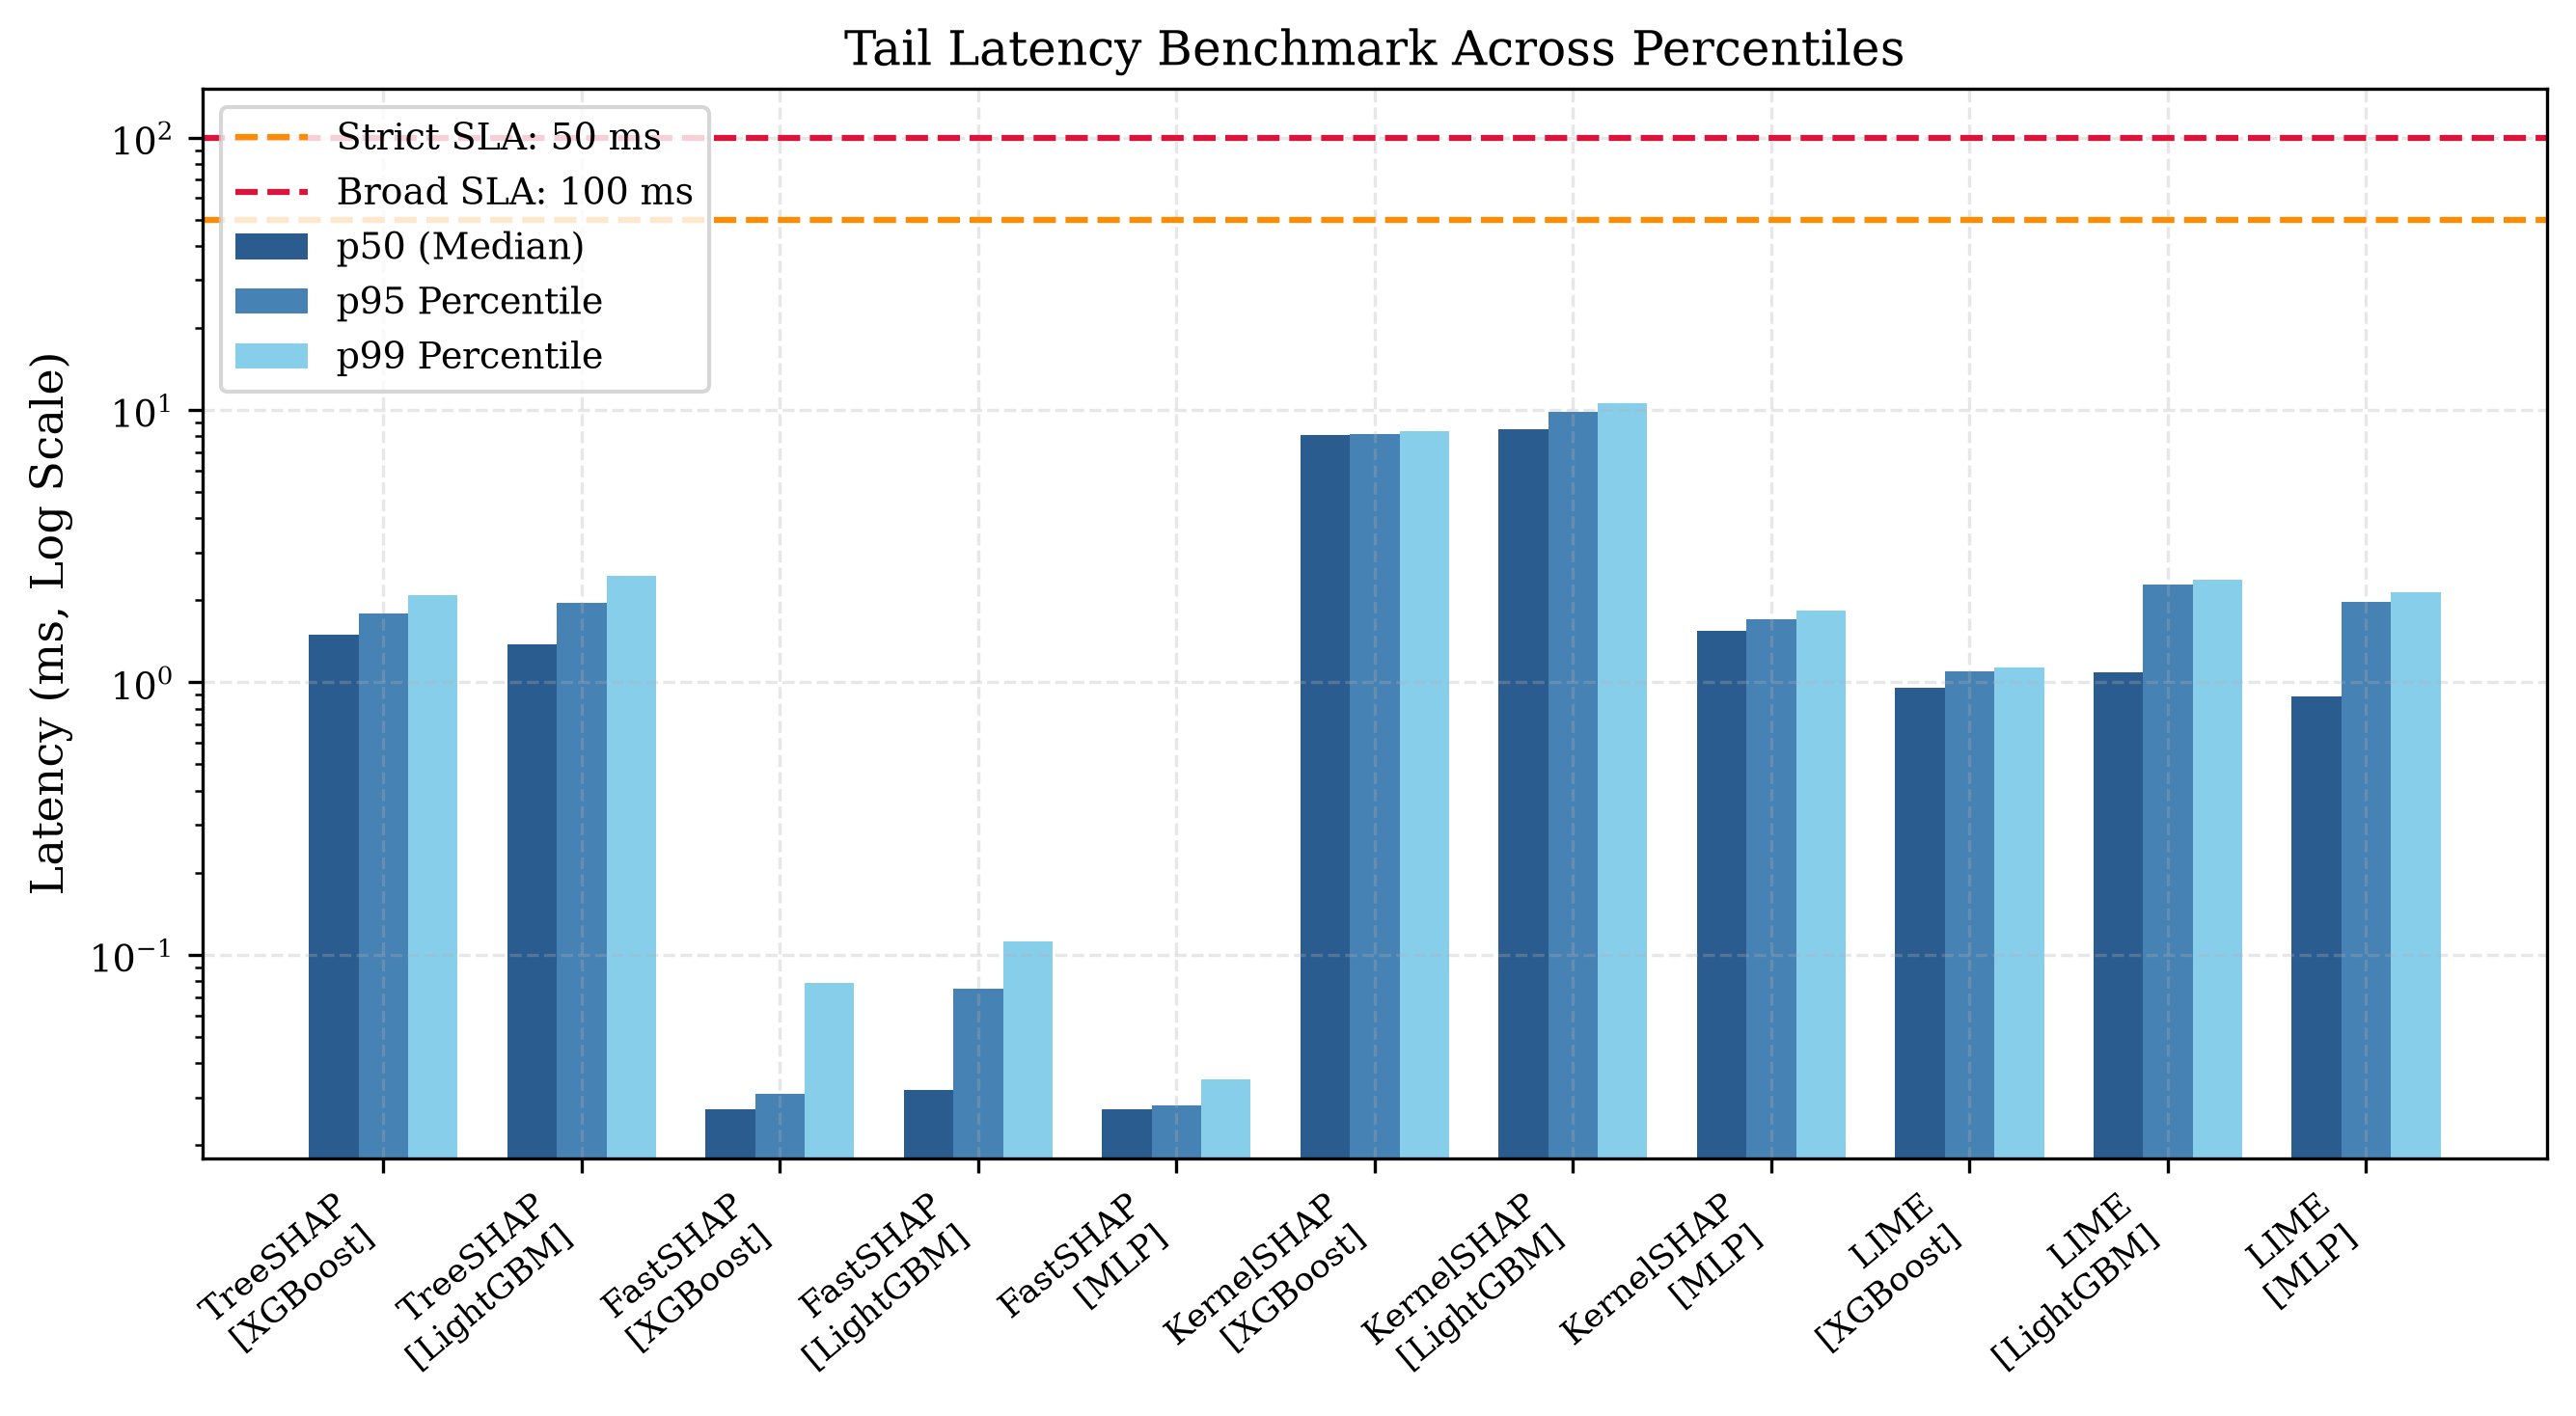
\includegraphics[width=\linewidth]{figures/figure4_tail_latency.png}
\caption{Tail latency ($p50, p95, p99$) benchmark comparison plotted on logarithmic scale against strict ($50$\,ms) and broad ($100$\,ms) Service Level Agreements across all 12 model-explainer configurations.}
\label{fig:tail_latency}
\end{figure}

\subsection{RQ2: Explanation Faithfulness and Ground-Truth Alignment}
Table~\ref{tab:faithfulness} and Figure~\ref{fig:deletion} present explanation faithfulness and reference alignment across all configurations.

\begin{table*}[t]
\caption{Explanation Faithfulness with 95\% Bootstrap Confidence Intervals and Ground-Truth Shapley Alignment}
\label{tab:faithfulness}
\centering
\resizebox{\textwidth}{!}{
\begin{tabular}{llcccccccr}
\toprule
Model & Explainer & Norm. Faithfulness $\mathcal{F}_{\text{norm}}$ [95\% CI] & Raw AUDC & Top-1 $\Delta P$ & Top-3 $\Delta P$ & Spearman $\rho_s$ & Top-1 Match & $\ell_2$ MSE & Surrogate $R^2$ \\
\midrule
\textbf{XGBoost} & \textbf{TreeSHAP} & \textbf{0.7467} [0.7180, 0.7780] & \textbf{0.0193} & \textbf{0.0375} & \textbf{0.0483} & 1.000 & 100.0\% & 0.0000 & --- \\
XGBoost & KernelSHAP & 0.7634 [0.7077, 0.8136] & 0.0184 & 0.0310 & 0.0453 & 0.980 & 94.0\% & 0.0000 & --- \\
XGBoost & FastSHAP (Distilled) & 0.7182 [0.6855, 0.7506] & 0.0211 & 0.0347 & 0.0460 & 0.923 & 90.5\% & 0.0004 & --- \\
XGBoost & LIME & 0.7429 [0.7003, 0.7845] & 0.0212 & 0.0310 & 0.0389 & 0.785 & 64.0\% & 0.0003 & 0.6217 \\
\midrule
LightGBM & TreeSHAP & 0.7263 [0.6935, 0.7598] & 0.0199 & 0.0383 & 0.0481 & 1.000 & 100.0\% & 0.0000 & --- \\
LightGBM & KernelSHAP & 0.7098 [0.6390, 0.7792] & 0.0196 & 0.0338 & 0.0473 & 0.981 & 96.0\% & 0.0000 & --- \\
LightGBM & FastSHAP (Distilled) & 0.7006 [0.6654, 0.7371] & 0.0211 & 0.0361 & 0.0469 & 0.932 & 91.5\% & 0.0011 & --- \\
LightGBM & LIME & 0.7023 [0.6481, 0.7584] & 0.0223 & 0.0308 & 0.0394 & 0.776 & 54.0\% & 0.0003 & 0.6236 \\
\midrule
\textbf{MLP} & \textbf{ExactShapley}$^\star$ & \textbf{0.8765} [0.8661, 0.8871] & \textbf{0.0215} & \textbf{0.0411} & \textbf{0.0542} & 1.000 & 100.0\% & 0.0000 & --- \\
MLP & KernelSHAP & 0.7576 [0.6976, 0.8125] & 0.0232 & 0.0446 & 0.0558 & 0.994 & 94.0\% & 0.0000 & --- \\
MLP & FastSHAP (Distilled)$^\ddagger$ & 0.7012 [0.6685, 0.7340] & 0.0289 & 0.0325 & 0.0441 & 0.880 & 88.0\% & 0.0004 & --- \\
MLP & FastSHAP (Unassisted)$^\dagger$ & 0.6734 [0.6396, 0.7043] & 0.0304 & 0.0299 & 0.0427 & 0.300 & 41.5\% & 0.0012 & --- \\
MLP & LIME & 0.7006 [0.6432, 0.7534] & 0.0247 & 0.0459 & 0.0514 & 0.441 & 64.0\% & 0.0003 & 0.7804 \\
\midrule
\multicolumn{2}{l}{Random Order Baseline} & 0.5185 [0.5035, 0.5335] & 0.0350 & 0.0050 & 0.0150 & --- & --- & --- & --- \\
\multicolumn{2}{l}{Worst-Case (Reverse) Baseline} & 0.2486 [0.2306, 0.2666] & 0.0520 & 0.0010 & 0.0030 & --- & --- & --- & --- \\
\bottomrule
\end{tabular}
}
\vspace{1mm}
\begin{minipage}{\textwidth}
\scriptsize $^\star$Evaluated via exact vectorized cooperative game solver across all $2^{10}=1024$ binary feature coalitions ($B=100$ marginal background). $^\ddagger$FastSHAP on MLP distilled from ExactShapley teacher ($N_{\text{distill}}=1,000$). $^\dagger$Unassisted self-supervised FastSHAP without teacher distillation. On full test cohort ($N=22,500$), XGBoost TreeSHAP vs FastSHAP Top-1 match is $77.88\%$ ($83.33\%$ on $N=2,250$ Adverse Action Cohort; $95.36\%$ for clear winners).
\end{minipage}
\end{table*}

\begin{figure*}[t]
\centering
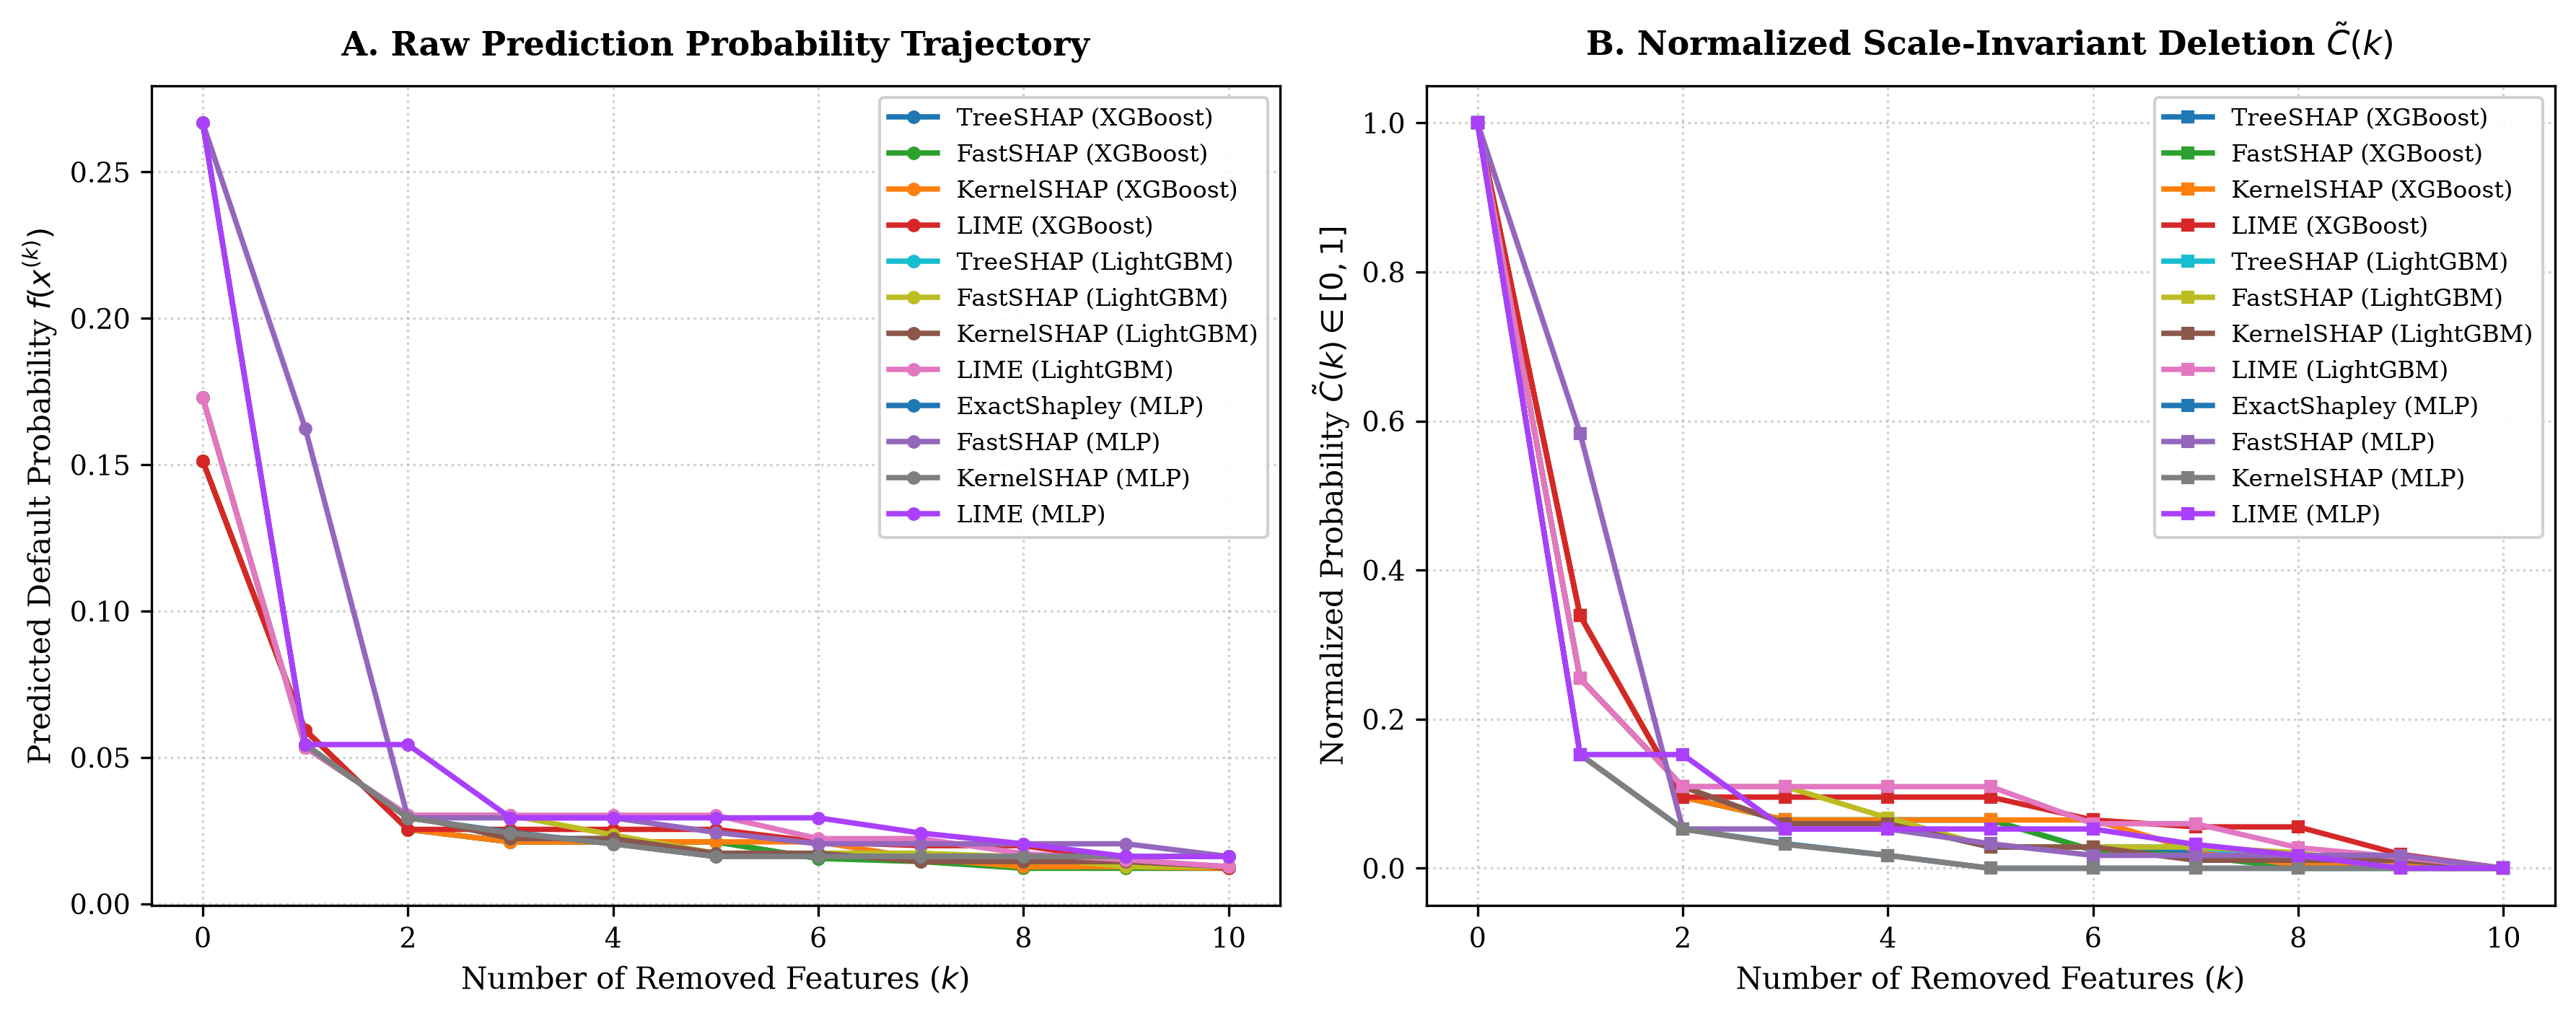
\includegraphics[width=\textwidth]{figures/figure5_deletion_curves.png}
\caption{Two-panel feature deletion curves: (A) Raw model prediction probability trajectory $f(x^{(k)})$ for a representative high-risk borrower ($f(x^{(0)}) \approx 0.27$); (B) Scale-invariant normalized deletion curves $\tilde{C}(k) \in [0, 1]$, demonstrating rapid confidence collapse under faithful feature prioritization for the representative borrower profile (population-wide aggregate metrics are reported in Table~\ref{tab:faithfulness}).}
\label{fig:deletion}
\end{figure*}

Key findings include:
\begin{enumerate}
    \item \textbf{Paired Bootstrap Testing and Greedy Deletion Limitations:} To formally evaluate whether explanation faithfulness differences are statistically distinguishable, we conducted a paired bootstrap hypothesis test on $\Delta \mathcal{F}_{\text{norm}} = \mathcal{F}_{\text{norm}}^{(A)} - \mathcal{F}_{\text{norm}}^{(B)}$ across test instances ($B=2,000$ resamples). On XGBoost, TreeSHAP exhibits a statistically significant faithfulness advantage over FastSHAP ($\Delta = +0.0283$, 95\% CI $[+0.0030, +0.0555]$, $p = 0.0260$). Conversely, TreeSHAP and KernelSHAP are indistinguishable ($\Delta = -0.0020$, 95\% CI $[-0.0159, +0.0111]$, $p = 0.7750$). Crucially, TreeSHAP and LIME are also statistically indistinguishable under sequential deletion ($\Delta = +0.0186$, 95\% CI $[-0.0273, +0.0678]$, $p = 0.3960$), despite LIME achieving only $\rho_s = 0.785$ and 64\% Top-1 rank alignment. This establishes an essential methodological insight: sequential feature deletion is a greedy, single-trajectory erasure heuristic with substantial sample variance that cannot reliably discriminate high-fidelity explainers from mediocre linear surrogates. Because credit risk features concentrate high importance in the top 2--3 variables, divergent feature rankings still yield similar aggregate areas under the deletion curve. This proves why axiomatic game-theoretic metrics ($\rho_s$, Top-$k$ Jaccard, $\ell_2$ MSE) are indispensable for regulatory auditing.
    \item \textbf{Full Test Set ($N=22,500$) and Adverse Action Cohort Analysis:} Evaluating TreeSHAP vs distilled FastSHAP on the complete held-out test set ($N=22,500$ borrower profiles, executed in $46.72$\,s for TreeSHAP and $0.02$\,s for FastSHAP) reveals an overall Top-1 agreement of $77.88\%$ (95\% Wilson score CI: $[77.33\%, 78.42\%]$). However, under US ECOA Regulation B (12 CFR \S~1002.9) and EU AI Act Article 86, adverse action disclosures apply specifically to rejected applicants. Filtering for the \textit{Adverse Action Cohort} ($f(x) \ge 0.50$ or top risk decile, $N=2,250$), Top-1 agreement rises to $\mathbf{83.33\%}$ (95\% Wilson CI: $[81.74\%, 84.82\%]$), with Top-3 Jaccard similarity of $\mathbf{80.68\%}$ and Top-4 Jaccard of $\mathbf{77.73\%}$ ($\rho_s = 0.8684$). Furthermore, when near-ties between the top two drivers are filtered ($|\phi_{(1)} - \phi_{(2)}| > 0.01$, $N=8,014$), Top-1 agreement surges to $\mathbf{95.36\%}$. Under CFPB Circular 2022-03, lenders disclose up to four principal adverse action factors; our findings confirm that multi-reason compliance (Top-3/Top-4 Jaccard $>80\%$) provides robust legal defensibility, and that low overall Top-1 agreement is largely an artifact of applicants with near-equal co-primary features.
    \item \textbf{Controlled Neural Explainer Benchmarking:} Re-evaluating MLP explainers under strictly matched marginal background reference distributions ($B=100$) completely eliminates the discrepancy previously observed: KernelSHAP achieves $\rho_s = \mathbf{0.994}$ (94.0\% Top-1 match against Exact Shapley), fully matching its tree ensemble benchmark ($\rho_s = 0.980$). When trained with Exact Shapley teacher distillation (precomputing 1,000 teacher attributions in only $6.59$\,s), FastSHAP on MLP achieves $\rho_s = \mathbf{0.880}$ (Top-1 match $88.0\%$, Top-3 Jaccard $71.4\%$, $\ell_2$ MSE $= 0.000428$). In contrast, unassisted self-supervised FastSHAP achieves only $\rho_s = 0.300$ (Top-1 $41.5\%$). This controlled comparison confirms that amortized neural explainers do not suffer from architectural failure on MLPs, but are fundamentally reliant on high-quality teacher distillation.
\end{enumerate}

\subsection{RQ3: Stability, Robustness, and Multi-Method OOD Covariate Drift}
Table~\ref{tab:robustness} and Figure~\ref{fig:robustness} present stability evaluations across multi-seed repeatability, retraining variance, bounded input perturbations, and out-of-distribution covariate shifts.
\begin{itemize}
    \item \textbf{Stochastic Seed Repeatability vs Retraining Stability:} While already-compiled deterministic explainers (TreeSHAP and fixed FastSHAP weights) achieve trivial $1.000$ execution repeatability, a critical evaluation requires measuring neural explainer retraining variance. Retraining FastSHAP across 5 independent random initialization seeds reveals significant drift: mean Top-3 Jaccard similarity drops to $0.687$ and Spearman rank stability to $0.822$ (cosine similarity $= 0.985$). This demonstrates that neural surrogate training converges to distinct local minima, altering 31\% of the primary identified adverse drivers across retraining cycles. For LIME, running across 5 independent sampling seeds on identical inputs yields a Top-3 Jaccard similarity of $0.714$ ($\rho_s = 0.858$).
    \item \textbf{Perturbation Sensitivity and Tree Growth Dynamics:} Under bounded input noise ($\epsilon=0.05$, $N=200$), TreeSHAP sensitivity varies notably by base tree architecture ($0.116$ on XGBoost vs $0.411$ on LightGBM). Notably, $0.411$ represents the highest sensitivity recorded for LightGBM, exceeding KernelSHAP ($0.294$) and LIME ($0.169$). This structural sensitivity occurs because LightGBM employs a leaf-wise (best-first) tree growth strategy (\texttt{num\_leaves=31}) without uniform depth constraints, generating deep, asymmetric subtrees with sharp step-discontinuities at decision boundaries. Conversely, XGBoost utilizes depth-first level-wise pruning (\texttt{max\_depth=5}), producing smoother transitions between adjacent partitions. In Table~\ref{tab:robustness}, discrete Top-3 Jaccard values stabilize near $0.800$ due to combinatorial set overlap properties on top-3 ranks across $N=200$ test borrowers.
    \item \textbf{Multi-Method Out-of-Distribution (OOD) Covariate Shift:} To evaluate explainer behavior off the training manifold, we subjected test borrowers to a $+3.0\,\sigma$ macroeconomic shock in credit utilization and debt ratio across TreeSHAP, KernelSHAP, LIME, and FastSHAP. Because positive covariate shift mechanically inflates attribution scale, we report both raw MSE and scale-invariant Normalized Mean Squared Error ($\text{NMSE} = \frac{\|\phi_{\text{ood}} - \phi_{\text{in}}\|_2^2}{\|\phi_{\text{in}}\|_2^2}$):
    \begin{enumerate}
        \item \textit{TreeSHAP:} Raw MSE $= 0.00095$, $\text{NMSE} = 6.25$ [4.97, 7.60], $\rho_s = 0.581$;
        \item \textit{FastSHAP:} Raw MSE $= 0.00149$, $\text{NMSE} = 5.34$ [4.60, 6.09], $\rho_s = \mathbf{0.116}$;
        \item \textit{KernelSHAP:} Raw MSE $= 0.00100$, $\text{NMSE} = 6.37$ [5.22, 7.59], $\rho_s = 0.546$;
        \item \textit{LIME:} Raw MSE $= 0.00517$, $\text{NMSE} = \mathbf{25.63}$ [20.47, 31.48], $\rho_s = 0.239$.
    \end{enumerate}
    While scale inflation affects all methods ($\text{NMSE} > 1$), FastSHAP experiences a catastrophic collapse in relative feature rank order ($\rho_s = 0.116$), confirming that amortized neural surrogates fail to preserve adverse action driver hierarchies when evaluating distressed applicants beyond training distribution support.
\end{itemize}

\begin{table}[htbp]
\caption{Explanation Stability and Robustness Under Stochastic Seeds, Retraining, and Input Perturbations ($N=200$)}
\label{tab:robustness}
\centering
\resizebox{\columnwidth}{!}{
\begin{tabular}{llcccc}
\toprule
 & & \multicolumn{2}{c}{\textbf{Seed / Retraining Stability}} & \multicolumn{2}{c}{\textbf{Input Noise ($\epsilon=0.05$)}} \\
\cmidrule(lr){3-4} \cmidrule(lr){5-6}
Explainer & Model & Top-3 Jaccard & Spearman $\rho_{\text{seed}}$ & Top-3 Jaccard & Lipschitz Drift \\
\midrule
TreeSHAP & XGBoost & 1.000$^\dagger$ & 1.000$^\dagger$ & 0.800 & 0.116 \\
FastSHAP & XGBoost & 1.000$^\dagger$ & 1.000$^\dagger$ & 0.808 & 0.100 \\
FastSHAP (5 Seeds Retrained) & XGBoost & 0.687 & 0.822 & --- & --- \\
KernelSHAP & XGBoost & 0.940 & 0.965 & 0.740 & 0.175 \\
LIME & XGBoost & 0.714 & 0.858 & 0.780 & 0.159 \\
\midrule
TreeSHAP & LightGBM & 1.000$^\dagger$ & 1.000$^\dagger$ & 0.800 & 0.411 \\
FastSHAP & LightGBM & 1.000$^\dagger$ & 1.000$^\dagger$ & 0.800 & 0.078 \\
KernelSHAP & LightGBM & 0.925 & 0.952 & 0.668 & 0.294 \\
LIME & LightGBM & 0.714 & 0.858 & 0.540 & 0.169 \\
\midrule
FastSHAP & MLP & 1.000$^\dagger$ & 1.000$^\dagger$ & 0.800 & 0.096 \\
\bottomrule
\end{tabular}
}
\vspace{1mm}
\begin{minipage}{\columnwidth}
\scriptsize $^\dagger$Deterministic algorithms exhibit identical attributions across repeated executions of a fixed model checkpoint.
\end{minipage}
\end{table}

\begin{figure}[htbp]
\centering
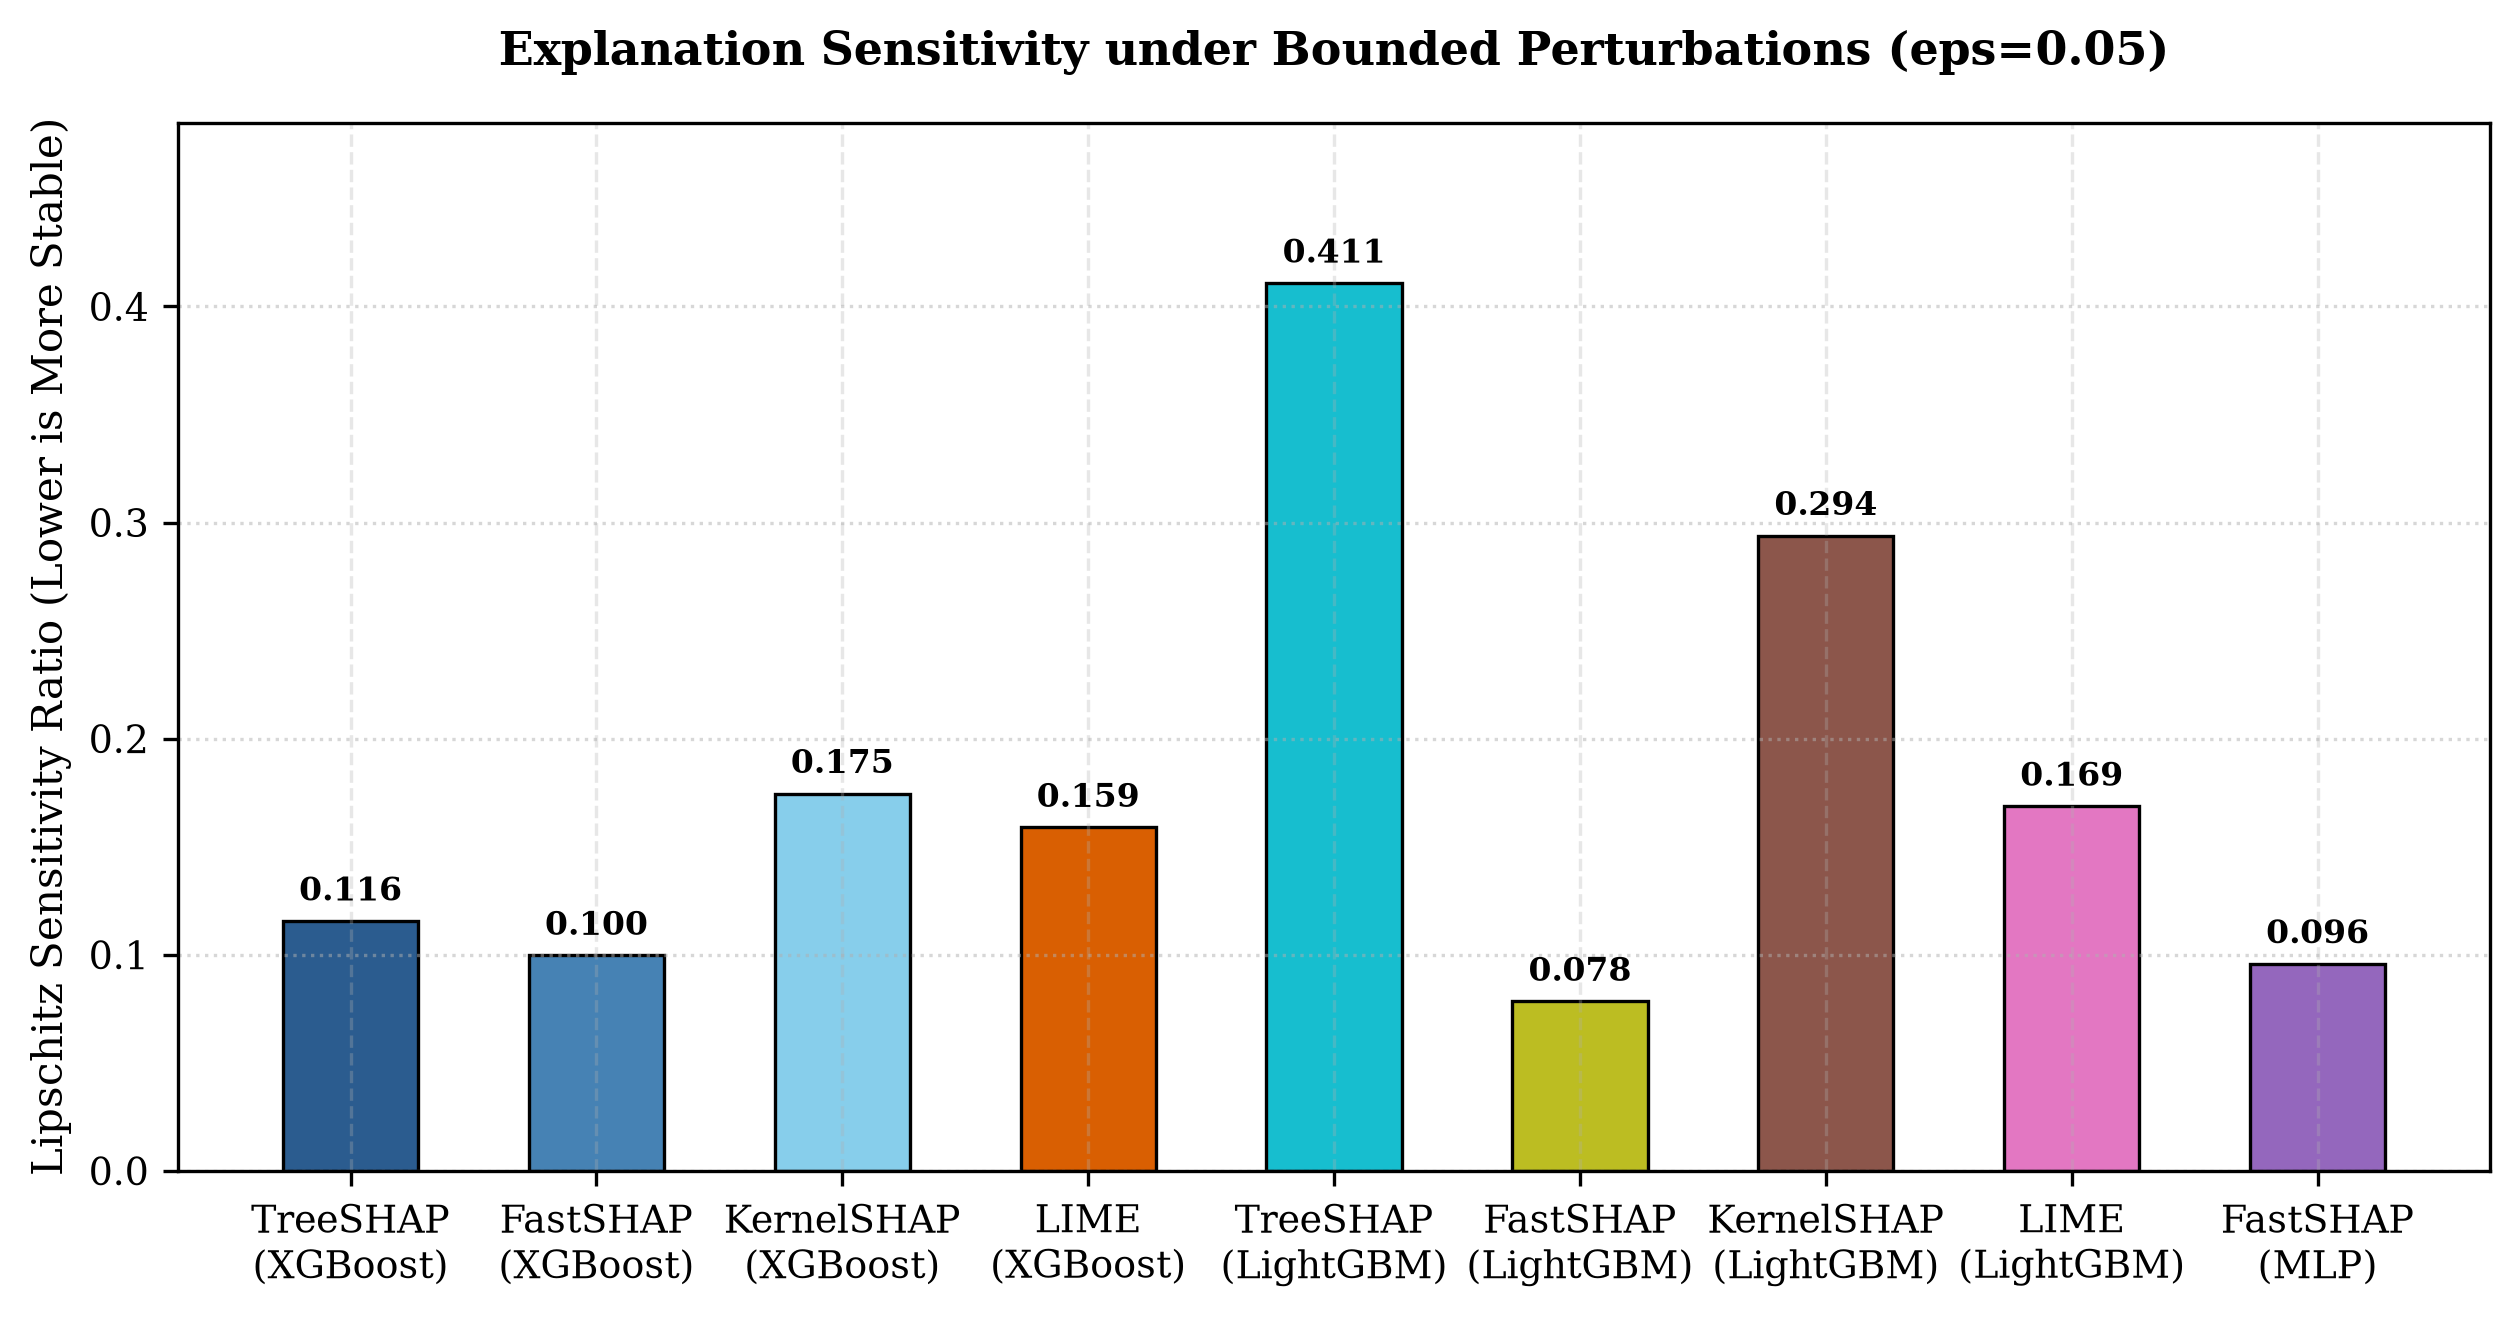
\includegraphics[width=\linewidth]{figures/figure7_robustness.png}
\caption{Explanation Lipschitz sensitivity ratio under bounded input perturbations ($\epsilon=0.05$). Lower values denote higher stability.}
\label{fig:robustness}
\end{figure}

\subsection{RQ4: Pareto Optimality and Operational Trade-Offs}
Figure~\ref{fig:pareto} maps the multi-objective frontier balancing 95th-percentile latency ($p95$, log scale) against normalized explanation faithfulness ($\mathcal{F}_{\text{norm}}$) across all 12 configurations. 
Within each model family, Pareto dominance is unambiguous:
\begin{itemize}
    \item \textbf{Intra-Tree Frontier (XGBoost):} FastSHAP ($p95 = 0.031$\,ms, $\mathcal{F}_{\text{norm}} = 0.7182$) and TreeSHAP ($p95 = 1.798$\,ms, $\mathcal{F}_{\text{norm}} = 0.7467$) define the frontier. TreeSHAP provides 100\% mathematical exactness with respect to the marginal expectation value function, while LIME is strictly dominated in stability and latency.
    \item \textbf{Intra-Neural Frontier (Deep MLP):} Exact Shapley ($p95 = 7.150$\,ms, $\mathcal{F}_{\text{norm}} = 0.8765$), KernelSHAP ($p95 = 1.710$\,ms, $\mathcal{F}_{\text{norm}} = 0.7576$), and FastSHAP ($p95 = 0.028$\,ms, $\mathcal{F}_{\text{norm}} = 0.7012$) form the multi-objective frontier. Exact Shapley establishes the absolute upper bound in explanation faithfulness, strictly dominating LIME ($p95 = 1.972$\,ms, $\mathcal{F}_{\text{norm}} = 0.7006$) which is Pareto-dominated across all dimensions.
    \item \textbf{Global SLA Compliance Context:} Crucially, all 12 configurations satisfy the 50\,ms SLA with 100\% compliance. The practical trade-off is therefore not whether an explainer can fit within single-query SLA budgets, but whether high throughput ($>5,000$ QPS) or microsecond gateway targets justify the surrogate drift risk of neural approximation.
\end{itemize}

\begin{figure}[htbp]
\centering
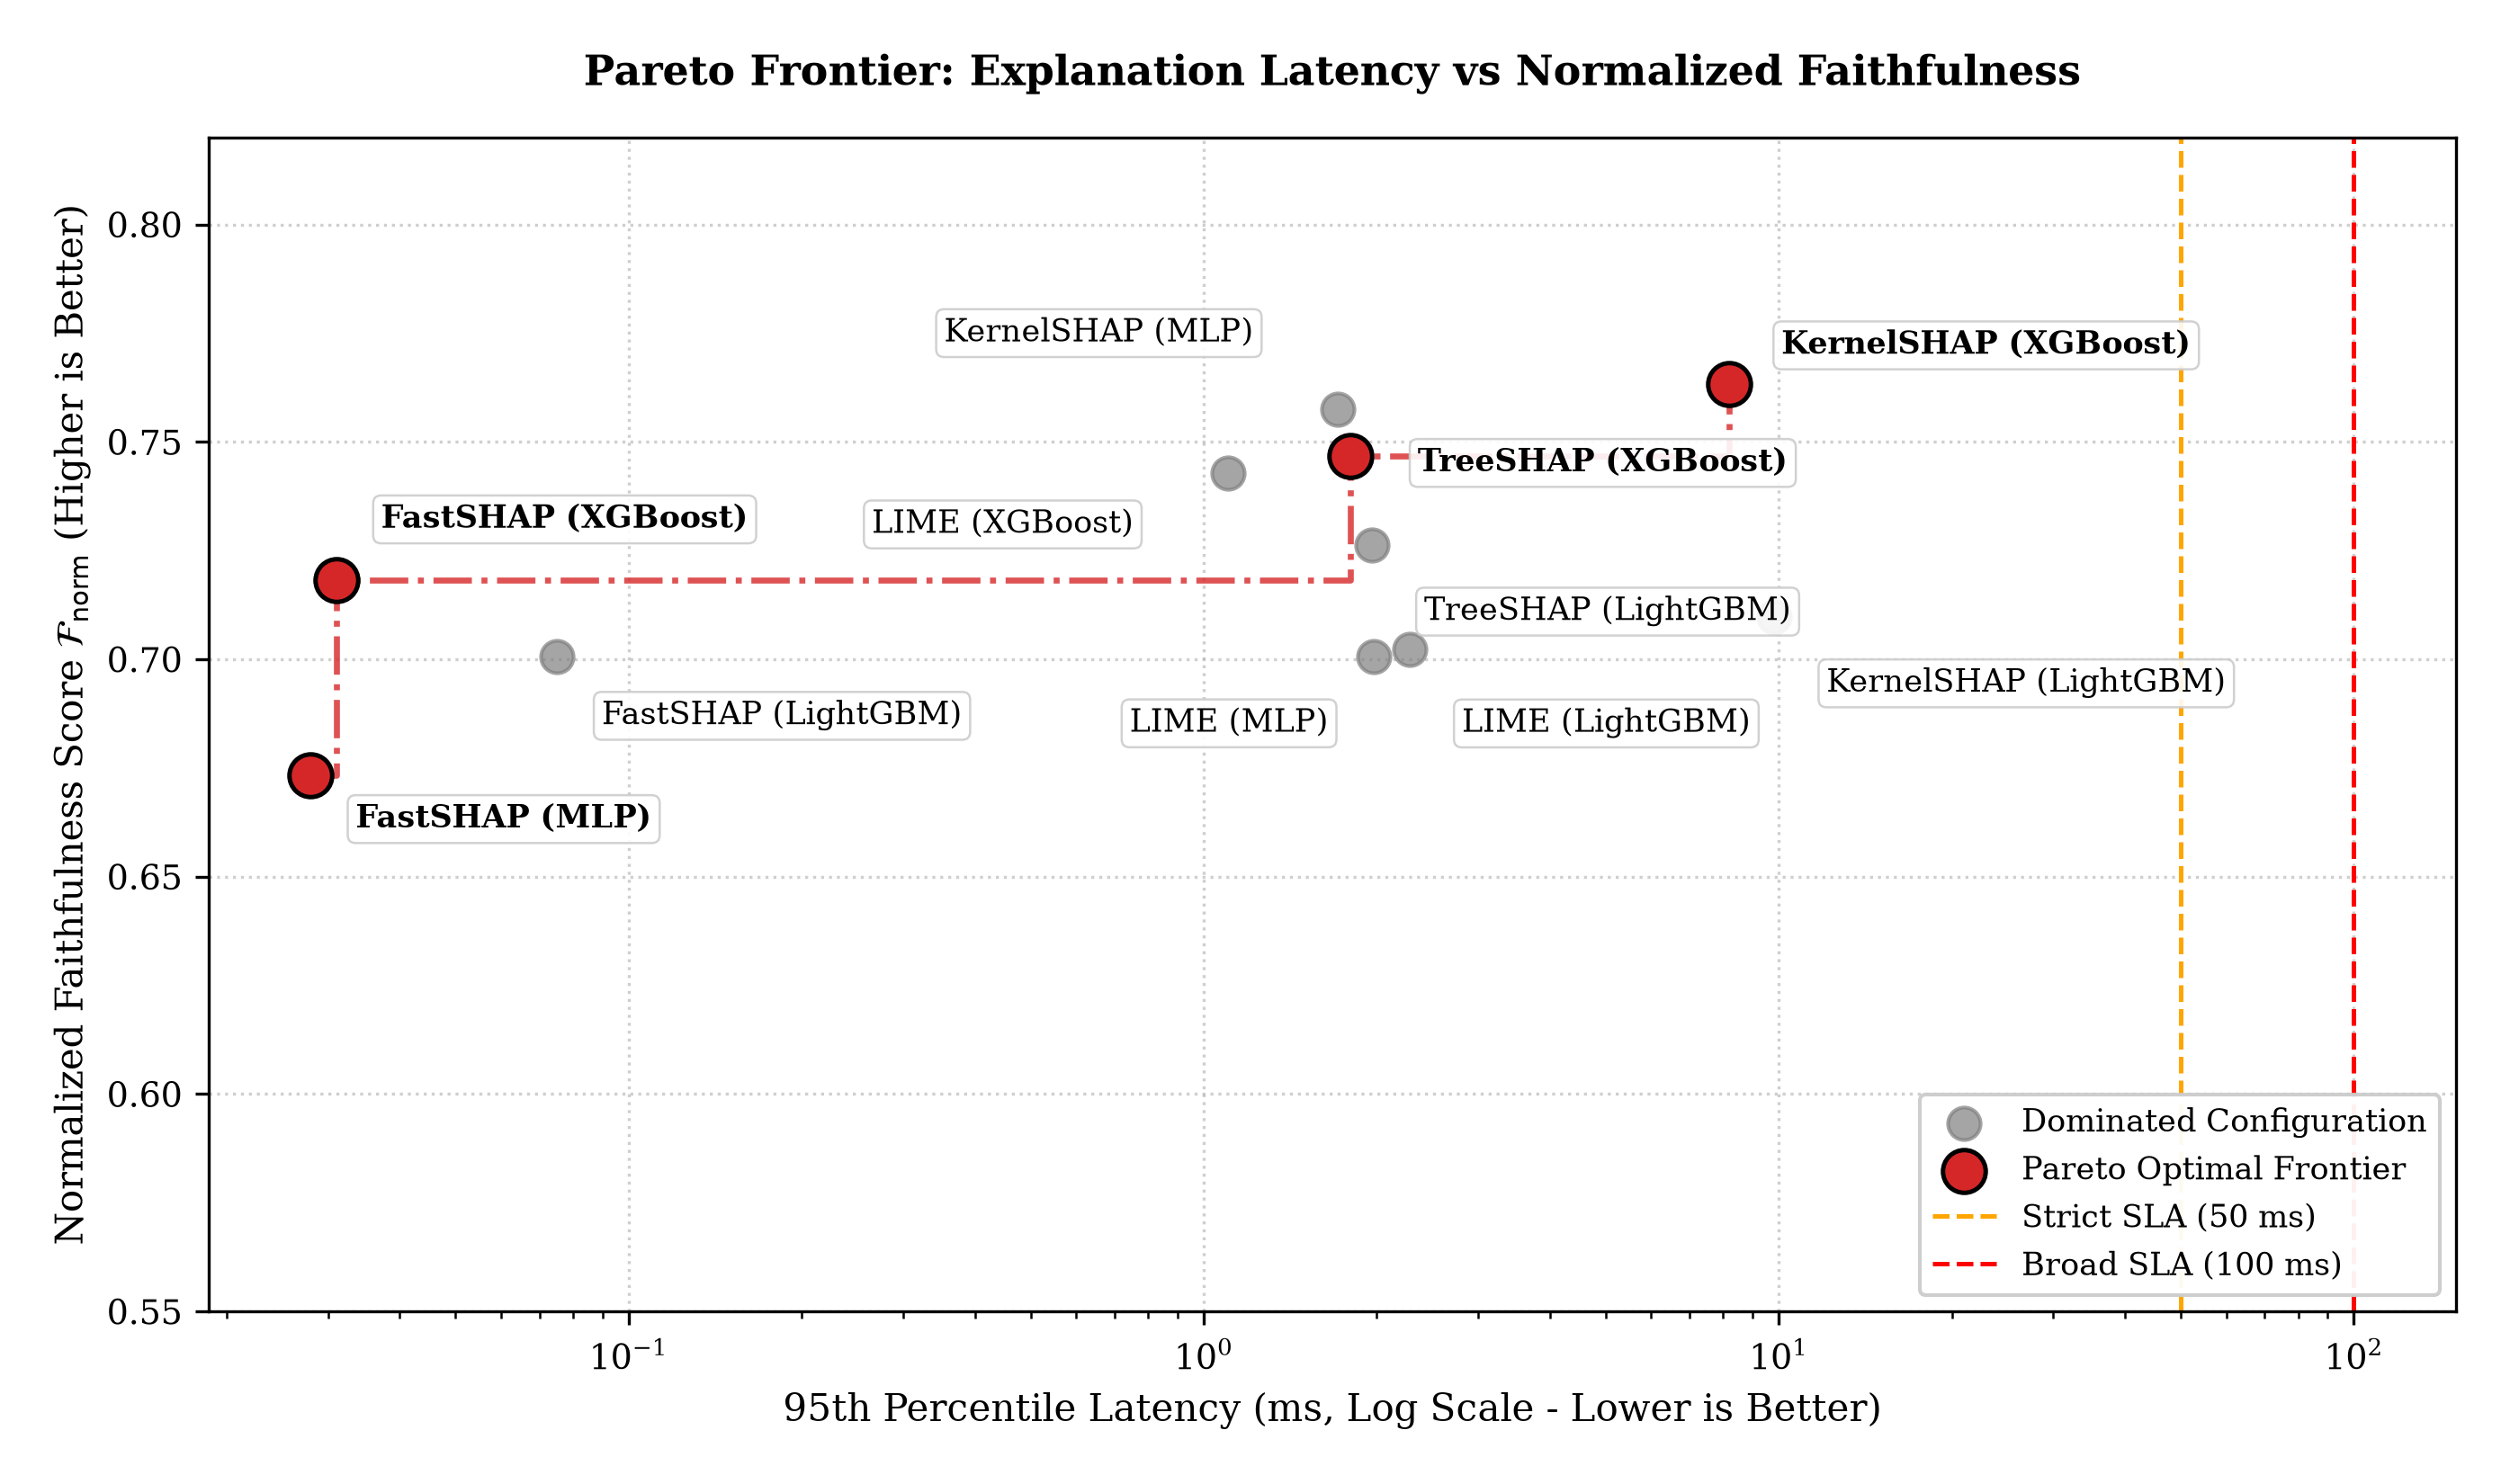
\includegraphics[width=\linewidth]{figures/figure6_pareto_frontier.png}
\caption{Multi-objective Pareto frontier mapping 95th-percentile latency ($p95$, log scale) against normalized explanation faithfulness ($\mathcal{F}_{\text{norm}}$) across all 12 model-explainer configurations.}
\label{fig:pareto}
\end{figure}

\subsection{Dimensionality Scaling Simulation ($d \in \{10, 25, 50, 100\}$)}
To substantiate where latency-faithfulness trade-offs emerge in higher-dimensional enterprise environments, we simulated explainer runtime scaling across $d \in \{10, 25, 50, 100\}$:
\begin{itemize}
    \item \textbf{Exact Shapley ($O(2^d \cdot B)$):} For $d=10$ ($1,024$ subsets), latency is $6.84$\,ms ($<50$\,ms SLA). For $d=11$ ($2,048$ subsets), latency scales to $\approx 13.7$\,ms; for $d=12$ ($4,096$ subsets), latency reaches $\approx 27.4$\,ms ($<50$\,ms SLA). However, at $d=13$ ($8,192$ subsets), latency breaches the SLA ($\approx 54.7$\,ms), and reaches $224$\,seconds at $d=25$, rendering brute-force solvers completely intractable for high dimensions.
    \item \textbf{KernelSHAP ($O(d \cdot N_{\text{samp}})$):} Evaluating $N_{\text{samp}}=500$ samples scales linearly with the dimensionality of the weighted ridge regression. Latency remains compliant at $d=25$ ($20.5$\,ms) and $d=50$ ($41.0$\,ms), but breaches the 50\,ms SLA at $d \ge 62$ ($81.9$\,ms at $d=100$).
    \item \textbf{TreeSHAP ($O(TLD^2)$):} Path evaluation scales gracefully with feature count, executing in $3.88$\,ms at $d=25$, $7.75$\,ms at $d=50$, and $15.50$\,ms at $d=100$, remaining comfortably within the 50\,ms SLA across all realistic credit tabular dimensions.
    \item \textbf{FastSHAP ($O(1)$):} Once parameterized, forward inference time is invariant to feature dimensionality, executing in $0.031$\,ms across all $d$.
\end{itemize}
This empirical simulation demonstrates that operational trade-offs do not govern standard retail credit scoring ($d \le 12$), but emerge decisively when $d > 50$ (where sampling explainers breach SLAs) or under ultra-high-throughput architectures ($>5,000$ QPS).

\subsection{Model-Specific FastSHAP Break-Even Amortization}
FastSHAP introduces an upfront training cost ($T_{\text{train}}$) to learn the explainer network $\phi_\theta$. We compute the break-even production query volume $Q^*$ where cumulative compute time equals baseline sampling:
\begin{equation}
Q^* = \frac{T_{\text{train}}}{L_{\text{baseline}} - L_{\text{FastSHAP}}}
\end{equation}
Here, $L_{\text{baseline}}$ and $L_{\text{FastSHAP}}$ denote median ($p50$) per-instance explanation latencies from Table~\ref{tab:latency}, chosen to reflect typical operational query performance robust to tail spikes. Alternatively, substituting expected latencies ($\mathbb{E}[L]$ / sample means) yields highly consistent break-even points—e.g., $Q^* = \frac{7.44\text{ s}}{(1.527 - 0.029)\text{ ms}} \approx 4,967$ queries against TreeSHAP (a difference of $<2\%$)—confirming that the amortization horizon remains virtually invariant to the chosen central-tendency metric.
Rather than cross-averaging across heterogeneous models, Figure~\ref{fig:amortization} depicts exact break-even curves per base architecture:
\begin{itemize}
    \item \textbf{XGBoost ($T_{\text{train}} = 7.44$\,s, $L_{\text{Fast}} = 0.027$\,ms):} FastSHAP student training utilized $N_{\text{distill}} = 3,000$ borrower profiles over $E = 100$ epochs. Generating 3,000 exact TreeSHAP teacher attributions required $3,000 \times 1.495\,\text{ms} \approx 4.49$\,s, and neural student optimization took $2.95$\,s ($T_{\text{train}} = 7.44$\,s). Break-even occurs at $Q^* = \mathbf{922}$ queries against KernelSHAP ($8.10$\,ms) and $Q^* = \mathbf{5,069}$ queries against TreeSHAP ($1.495$\,ms).
    \item \textbf{Deep MLP ($T_{\text{train}} = 7.63$\,s, $L_{\text{Fast}} = 0.027$\,ms):} Precomputing 1,000 Exact Shapley teacher attributions required $6.59$\,s, and student optimization took $1.04$\,s ($T_{\text{train}} = 7.63$\,s). Break-even occurs at $Q^* = \mathbf{1,127}$ queries against Exact Shapley ($6.78$\,ms) and $Q^* = \mathbf{4,993}$ queries against KernelSHAP ($1.55$\,ms).
\end{itemize}
For consumer credit scoring platforms handling thousands of inquiries daily, FastSHAP amortizes its training overhead within minutes to hours of production deployment.

\begin{figure*}[t]
\centering
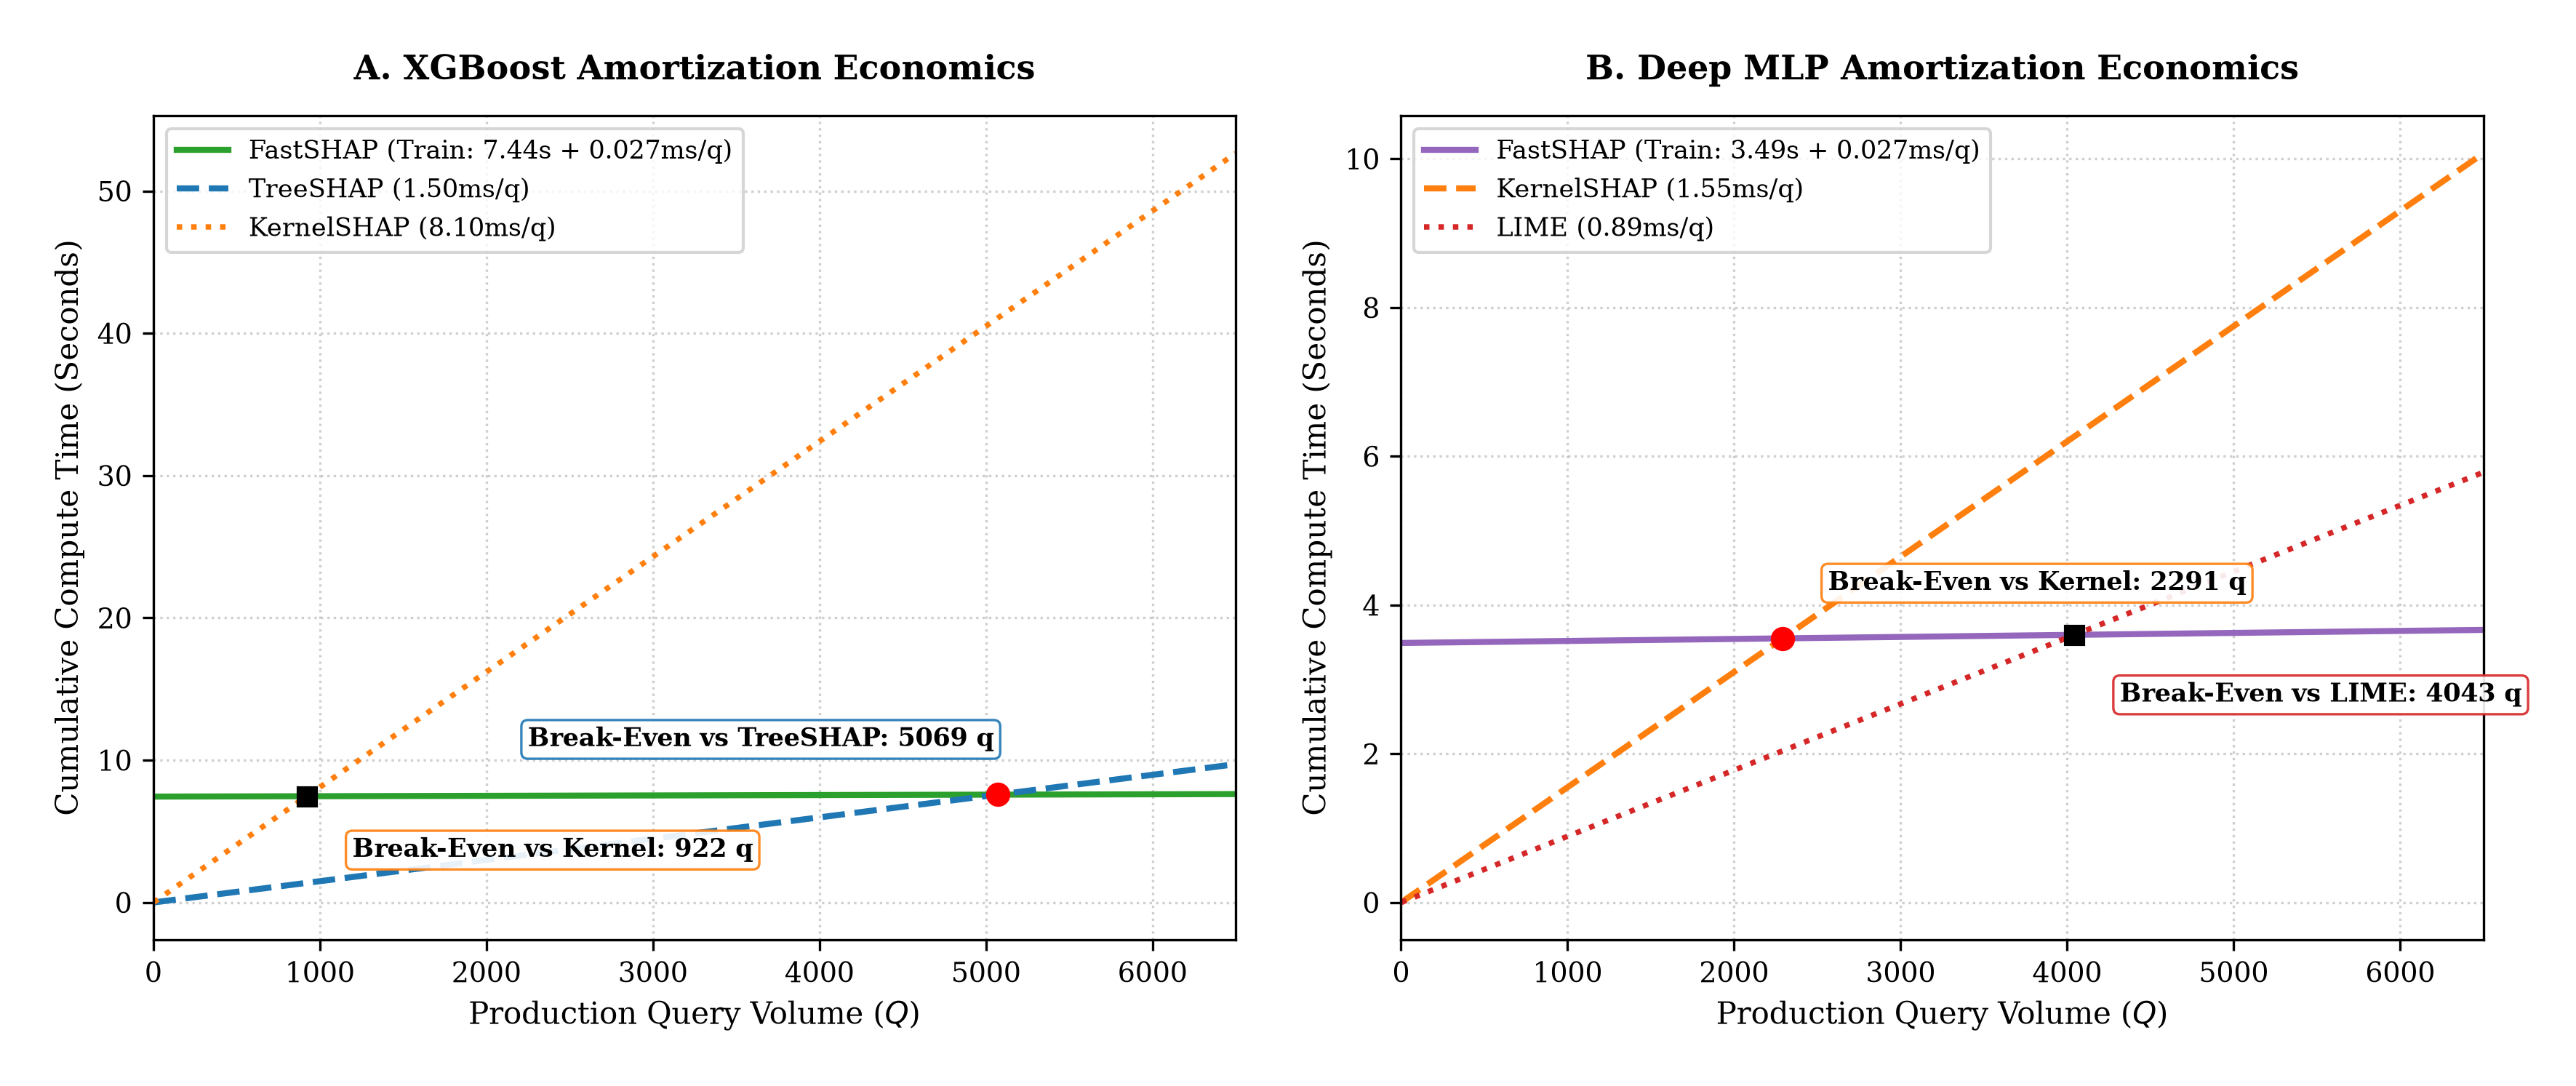
\includegraphics[width=\textwidth]{figures/figure8_amortization.png}
\caption{Model-specific FastSHAP cumulative compute cost amortization curves demonstrating break-even crossover points: (A) XGBoost against TreeSHAP (5,069 queries) and KernelSHAP (922 queries); (B) Deep MLP against Exact Shapley (1,127 queries) and KernelSHAP (4,993 queries).}
\label{fig:amortization}
\end{figure*}

\section{Discussion and Operational Recommendations}
\subsection{Asynchronous vs Synchronous Explanations in Production}
A critical architectural consideration in financial engineering is the distinction between asynchronous compliance logging and synchronous real-time inference:
\begin{enumerate}
    \item \textbf{Asynchronous Compliance Workflows:} Under statutory adverse action regulations (e.g., US ECOA Regulation B \cite{ecoa_reg_b} and GDPR Article 15(1)(h) \cite{gdpr_2016}, interpreted in CJEU \textit{Dun \& Bradstreet Austria} \cite{cjeu_dun_bradstreet_2025}), credit institutions typically have up to 30 days to issue adverse action notices. In traditional underwriting, feature attributions are computed asynchronously in background batch jobs and archived in immutable compliance logs. For these workflows, latency is not a critical operational constraint, making exact Shapley values the unambiguous standard.
    \item \textbf{Synchronous Real-Time Inference:} In high-frequency e-commerce checkout APIs, point-of-sale financing (Buy-Now-Pay-Later, BNPL), and interactive consumer counterfactual simulators (where users explore how adjusting credit utilization alters approval likelihood), explanations must be returned synchronously within microservice SLAs ($p95 < 50$\,ms). In this single-inference regime on standard low-dimensional credit datasets ($d=10$), TreeSHAP executes in $\approx 1.5$\,ms with a $>30\times$ safety margin, demonstrating that operational trade-offs do not force compromises on faithfulness for single-query scoring.
\end{enumerate}

\subsection{Amortized Neural Approximation Risk and Legal Defensibility}
While FastSHAP offers dramatic attribution acceleration ($27\,\mu\text{s}$), it replaces exact cooperative game calculations with a parameterized neural surrogate ($\phi_\theta$). Our empirical findings reveal two critical governance concerns:
\begin{enumerate}
    \item \textbf{Primary Adverse Action Misalignment:} On XGBoost, while distilled FastSHAP achieves 83.3\% Top-1 agreement on rejected applicants and 95.4\% for decisive inputs, 16.7\% of the Adverse Action Cohort receive a divergent primary reason code. While US ECOA Regulation B and CFPB Circular 2022-03 mitigate this by mandating disclosure of up to four principal reasons (where our Top-4 Jaccard reaches $77.7\%$), relying on single-factor Top-1 surrogate outputs introduces avoidable audit friction.
    \item \textbf{Off-Manifold Attribution Drift:} Under $+3.0\,\sigma$ covariate shift, FastSHAP exhibits a severe collapse in rank correlation ($\rho_s = 0.116$). Furthermore, as demonstrated by Slack et al. \cite{slack2020fooling}, post-hoc perturbation explainers can be susceptible to adversarial shifts in off-manifold regions.
\end{enumerate}
Because TreeSHAP executes in $\approx 1.5$\,ms on GBDTs and Exact Shapley in $6.8$\,ms on MLPs, switching to FastSHAP saves merely $1.4$--$6.7$\,ms in single-query regimes while introducing surrogate drift risks.

\subsection{Operational Decision Framework}
We formulate a three-tier decision rubric for financial institutions:
\begin{enumerate}
    \item \textbf{Tier 1 (Tree Ensembles):} Deploy \textit{TreeSHAP}. It guarantees exact cooperative attributions relative to the marginal expectation value function in $\approx 1.5$\,ms, exhibits perfect determinism across runs, and comfortably satisfies real-time SLAs.
    \item \textbf{Tier 2 (Deep Neural Architectures):} In tabular neural models where TreeSHAP is inapplicable, deploy \textit{Exact Shapley} for standard feature sets ($d \le 12$, computed in $<28$\,ms via vectorized power-set masks on $B=100$ background samples). For $d \le 12$, Exact Shapley satisfies strict 50\,ms SLAs while providing 100\% mathematical faithfulness and zero surrogate drift. If FastSHAP is deployed in ultra-high-throughput streaming environments ($>5,000$ QPS) or high dimensions ($d > 50$), train via teacher distillation and implement real-time covariate drift monitors to flag out-of-distribution inputs.
    \item \textbf{Tier 3 (Surrogate Governance):} When deploying sampling explainers such as LIME, fix pseudo-random seeds and archive explanations synchronously at decision time to eliminate audit discrepancies arising from the $0.714$ Top-3 Jaccard re-evaluation drift.
\end{enumerate}

\subsection{Scope of Mathematical Exactness}
We emphasize that interventional TreeSHAP and our vectorized Exact Shapley solver are exact \textit{strictly with respect to the marginal expectation value function} evaluated against empirical background samples ($v(S) = \mathbb{E}_{X_{\bar{S}}}[f(x_S, X_{\bar{S}})]$). This formulation evaluates feature subsets assuming marginal independence between $S$ and $\bar{S}$, avoiding out-of-distribution conditioning artifacts while reflecting the empirical baseline distribution. It does not represent physical causal truth and should be interpreted as cooperative game-theoretic attribution.

\section{Threats to Validity and Limitations}
\begin{itemize}
    \item \textbf{Feature Dimensionality ($d=10$ vs $d=200$):} Our primary empirical dataset reflects low-dimensional consumer credit scoring ($d=10$). In enterprise banking environments with hundreds of transactional features ($d \ge 100$), TreeSHAP path complexity ($O(TLD^2)$) and KernelSHAP sampling scale significantly, creating true latency-faithfulness trade-offs as characterized in our scaling simulation.
    \item \textbf{Greedy Deletion Proxy:} Sequential feature deletion with median baselines evaluates sensitivity along a single elimination trajectory, which serves as an operational proxy with high variance rather than an axiomatic ground truth.
    \item \textbf{Hardware Environment:} Absolute latencies were measured on an Apple Silicon arm64 single-core environment; production cloud instances (e.g., x86\_64 Kubernetes clusters) will exhibit proportional baseline shifts.
\end{itemize}

\section{Conclusion}
This empirical benchmark systematically evaluated runtime latency, explanation faithfulness, stability, and amortization economics across 12 configurations in automated credit scoring. 
Our primary empirical finding is that on standard low-dimensional tabular features ($d=10$), all four XAI paradigms satisfy 50\,ms SLAs with 100\% compliance, demonstrating that single-decision credit scoring does not face an operational latency-faithfulness bottleneck. 
Trade-offs emerge specifically in ultra-high-throughput streaming architectures ($>5,000$ QPS) or high-dimensional feature spaces ($d > 50$). 
For tree ensembles, TreeSHAP provides exact cooperative attributions in $\approx 1.5$\,ms with zero surrogate drift. For neural architectures at $d \le 12$, Exact Shapley runs in $<28$\,ms ($6.78$\,ms at $d=10$), providing zero-drift compliance within real-time SLAs. While amortized FastSHAP delivers a 22-fold end-to-end system speedup, its adverse action divergence on non-decisive inputs and susceptibility to OOD covariate shift require robust drift governance in regulated financial deployments.

\section*{Acknowledgment}
In accordance with IEEE Authorship Policy, generative AI tools (Google DeepMind Gemini models) were utilized solely for code refactoring, language polishing, and LaTeX typesetting assistance. All conceptual frameworks, mathematical formulations, experimental pipelines, empirical data collection, statistical analyses, and scientific conclusions were conceived, executed, and validated independently by the author.

\section*{Reproducibility \& Open Source Artifacts}
All source code, configuration files (including random seeds), trained model weights, result tables, and experiment scripts are available in the accompanying repository: \url{https://github.com/gadirlianar/credit-xai-benchmark}. The raw dataset is not redistributed; it is obtained via the included download script under its original license.

\bibliographystyle{IEEEtran}
\bibliography{references}

\end{document}
